\documentclass[letterpaper,oneside]{book}
%\documentclass[letterpaper,twoside]{book}
% the two-column setup looks better for letter paper with a larger width.
\usepackage{geometry}
\geometry{margin=1.5cm, vmargin={0pt,1cm}}
\setlength{\topmargin}{-1cm}
\setlength{\paperheight}{29.7cm}
\setlength{\textheight}{25.1cm}

% auto adjust the marginals
\usepackage{marginfix}

\usepackage[algo2e,lined,boxed,linesnumbered]{algorithm2e}
\usepackage{amsfonts}
\usepackage{amsmath}
\usepackage{amssymb}
\usepackage{amsthm}
%\usepackage{CJKutf8}
\usepackage{enumerate}
\usepackage{fancyhdr}
\usepackage{graphicx}
\usepackage{float}
\usepackage{layout}
\usepackage{lineno}
\usepackage{makeidx}
\usepackage{mathrsfs}
\usepackage[version=4]{mhchem}
\usepackage{lipsum}
\usepackage{multicol,caption}
\usepackage{natbib}
\usepackage{subfigure}
\usepackage{tcolorbox} % this package is needed for \voidenvironment below
\usepackage{tikz}
\usetikzlibrary{arrows,automata,backgrounds,cd}
\usetikzlibrary{shapes,snakes}

\newcommand{\Rx}[1]{\mathrm{R}[#1]}
\newcommand{\Lx}[1]{\mathrm{L}[#1]}
\newcommand{\Ux}[1]{\mathrm{U}[#1]}
\newcommand{\Dx}[1]{\mathrm{D}[#1]}
\newcommand{\Cx}[1]{\mathrm{C}[#1]}
\newcommand{\Sx}[1]{\mathrm{S}[#1]}
\newcommand{\norm}[1]{\|#1\|}
\newcommand{\ccg}[1]{\overline{#1}}
\newcommand{\dif}{\mathrm{d}}
\newcommand{\Dim}{\mathrm{D}}
\newcommand{\avg}[1]{\left\langle #1 \right\rangle}
\newcommand{\innerProd}[1]{\left\langle #1 \right\rangle}
\newcommand{\cond}{\mathrm{cond}}
\newcommand{\Cond}[2]{\mathrm{cond}_{#1}\left(#2\right)}
\newcommand{\difFrac}[2]{\frac{\dif #1}{\dif #2}}
\newcommand{\gen}[1]{\left\langle #1 \right\rangle}
\newcommand{\ii}{\mathbf{i}}
\newcommand{\Imz}{\mathrm{Im}\,}
\newcommand{\Int}{\mathrm{Int}}
\newcommand{\Ext}{\mathrm{Ext}}
\newcommand{\Cl}{\mathrm{Cl}}
\newcommand{\Fr}{\mathrm{Fr}}
\newcommand{\Ker}{\mathrm{ker}}
\newcommand{\pdfFrac}[2]{\frac{\partial #1}{\partial #2}}
\newcommand{\Rez}{\mathrm{Re}\,}
\newcommand{\sgn}{\mathrm{sgn}}
\newcommand{\Span}{\mathrm{span}}
\newcommand{\OFL}{\mathrm{OFL}}
\newcommand{\UFL}{\mathrm{UFL}}
\newcommand{\fl}{\mathrm{fl}}
%\newcommand{\op}{\mathrm{op}}
\newcommand{\op}{\odot}
\newcommand{\Eabs}{E_{\mathrm{abs}}}
\newcommand{\Erel}{E_{\mathrm{rel}}}
\newcommand{\dom}{\mathrm{dom}}
\newcommand{\Null}{\mathrm{null}}
\newcommand{\Range}{\mathrm{range}}
\newcommand{\Supp}{\mathrm{supp}}
\newcommand{\Arity}{\mathrm{arity}}

\newenvironment{Figure}
{\par\medskip\noindent\minipage{\linewidth}}
{\endminipage\par\medskip}

% this environment is for solutions of examples and exercises
\newenvironment{solution}%
{\noindent\textbf{Solution.}}%
{\qedhere}
% the following command is for disabling environments
%  so that their contents do not show up in the pdf.
\makeatletter
\newcommand{\voidenvironment}[1]{%
  \expandafter\providecommand\csname env@#1@save@env\endcsname{}%
  \expandafter\providecommand\csname env@#1@process\endcsname{}%
  \@ifundefined{#1}{}{\RenewEnviron{#1}{}}%
}
\makeatother



%----------------------------------------
% theorem and theorem-like environments %
%----------------------------------------
\numberwithin{equation}{chapter}
\theoremstyle{definition}

\newtheorem{thm}{Theorem}[chapter]
\newtheorem{alg}[thm]{Algorithm}
\newtheorem{asm}[thm]{Assumption}
\newtheorem{axm}[thm]{Axiom}
\newtheorem{coro}[thm]{Corollary}
\newtheorem{defn}[thm]{Definition}
%\newtheorem{exm}{Example}[chapter]
%\newtheorem{exc}[exm]{Exercise}
% number examples and exercises with thms.
\newtheorem{exm}[thm]{Example}
\newtheorem{exc}[thm]{Exercise}
\newtheorem{frm}[thm]{Formula}
\newtheorem{lem}[thm]{Lemma}
\newtheorem{ntn}{Notation}
\newtheorem{prop}[thm]{Proposition}
\newtheorem{rem}{Remark}[chapter]
\newtheorem{rul}[thm]{Rule}


%%%%%%%%%%%%%% for INSE %%%%%%%%%%%%%
\usepackage{bm}
\usepackage[sans]{dsfont}
\usepackage{url}
\newcommand{\ibold}{{\mathbf{i}}}
\newcommand{\jbold}{{\mathbf{j}}}
\newcommand{\kbold}{{\mathbf{k}}}
\newcommand{\ebold}{{\mathbf{e}}}
\newcommand{\ubold}{{\mathbf{u}}}
\newcommand{\xbold}{{\mathbf{x}}}
\newcommand{\pbold}{{\mathbf{p}}}
\newcommand{\etabold}{\bm{\eta}}
\newcommand{\unitV}{\mathds{1}}
\newcommand{\zerobold}{{\mathbf{0}}}
\newcommand{\dt}{{\Delta t}}
\newcommand{\avgI}[1]{\langle #1 \rangle_{\ibold}}
\newcommand{\iphed}{{\ibold+\frac{1}{2}\ebold^d}}
\newcommand{\imhed}{{\ibold-\frac{1}{2}\ebold^d}} %new
% i plus fractional e^d
\newcommand{\ipfed}[1]{\ibold+\frac{#1}{2}\ebold^d}
% i minus fractional e^d
\newcommand{\imfed}[1]{\ibold-\frac{#1}{2}\ebold^d}
\newcommand{\ipmfed}[1]{\ibold\pm\frac{#1}{2}\ebold^d}
\newcommand{\half}{\frac{1}{2}}
\newcommand{\Lapl}{{\mathbf{L}}}
\newcommand{\Div}{{\mathbf{D}}}
\newcommand{\Grad}{{\mathbf{G}}}
\newcommand{\Iden}{{\mathbf{I}}}
\newcommand{\nref}{n_{\text{ref}}}
\newcommand{\phio}{\phi^{\circ}}
\newcommand{\eq}[1]{(\ref{#1})}
\newcommand{\Proj}{{\mathbf{P}}}
\newcommand{\cProj}{{\mathcal{P}}}
\newcommand{\cProjLH}{{\mathscr{P}}}
\newcommand{\ProjAux}{{\mathbf{Q}}}
\newcommand{\exOp}{{\mathbf{X}}^{[\text{E}]}}
\newcommand{\imOp}{{\mathbf{X}}^{[\text{I}]}}
\newcommand{\nStages}{n_{\tiny \textsf{s}}}
\newcommand{\Sc}{\mathcal{S}}
\newcommand{\M}{\mathcal{M}}
\newcommand{\cp}[2]{\cup_{#1=1}^{#2}}
\newcommand{\sm}[2]{\sum_{#1=1}^{#2}}
%%%%%%%%%%%%%%%%%%%%%%%%%%%%%%%%%
\newcommand{\fYear}{2024}


%\makeindex
  
\begin{document}
\pagenumbering{roman}

%\thispagestyle{empty}
\begin{small}
\tableofcontents
\end{small}

% --------------------------------------------------------
% uncomment the following to remove these environments 
%  to generate handouts for students.
% --------------------------------------------------------
\begingroup
%\voidenvironment{rem}%
%\voidenvironment{proof}%
%\voidenvironment{solution}%
% \input{sec/methodsOfStudy}

%\setcounter{chapter}{-1}
\pagenumbering{arabic}

\setcounter{page}{1}

%\clearpage

% This page has been intentionally left blank.

% \clearpage

\pagestyle{fancy}
\fancyhead{}
\lhead{Shuang Hu, Linwei Wu}
\chead{Real Analysis}
\rhead{\fYear}

% \input{sec/part-I}

% \pagestyle{fancy}
% \fancyhead{}
% \lhead{Qinghai Zhang}
% \chead{Numerical Solutions of Differential Equations}
% \rhead{\fYear}

% \input{sec/part-II}

% \input{sec/part-III}

%\appendix

\pagestyle{fancy}
\fancyhead{}
\lhead{Shuang Hu,Linwei Wu}
\chead{Measures}
\rhead{\fYear}

\chapter{Measures}
\label{cha:measures}

\begin{multicols}{2}
\setlength{\columnseprule}{0.2pt}  

\section{Introduction}
\begin{exm}
    The \textbf{length} of an interval 
    $[a,b]\subset\mathbb{R}$ is $b-a$.
\end{exm}
\begin{exm}
    The \textbf{area} of a rectangle 
    $[a_1,b_1]\times [a_2,b_{2}]\subset\mathbb{R}^{2}$ 
    is $(b_1-a_1)(b_2-a_2)$.
\end{exm}
\begin{exm}
    The \textbf{volume} of a cube 
    $[a_1,b_1]\times [a_2,b_2]\times [a_3,b_3]\subset\mathbb{R}^3$ 
    is $(b_1-a_1)(b_2-a_2)(b_3-a_3)$.
\end{exm}
\begin{rem}
    The length, area and volume have something in common. 
    They are all derived by the \textbf{size} of 
    a subset $\Sc\subset\mathbb{R}^{n}$. 
    Then, for $X=\mathbb{R}^n$, we can give the `volume' 
    of a subset $\Sc\subset X$ with some necessary properties.  
\end{rem}
\begin{ntn}
    For a set $\Sc$, we denote 
    \begin{displaymath}
        \mathcal{P}(\Sc):=\{\M:\M\subset\Sc\}.
    \end{displaymath}
\end{ntn}
\begin{defn}
    \label{Defn:volume}
    In $\mathbb{R}^{n}$, the \textit{volume} is a function 
    $\mu:\mathcal{D}\subset 
    \mathcal{P}(\mathbb{R}^{n})\rightarrow\mathbb{R}$ satisfies:
    \begin{itemize}
        \item For a sequence $\{E_{i}\}_1^{\infty}\subset\mathcal{D}$ 
        and $\forall i\neq j$, $E_i\cap E_{j}=\emptyset$, 
        $\mu(\cp{i}{\infty}E_{i})=\sm{i}{\infty}\mu(E_i)$.
        \item If $E\subset F$, then $\mu(E)\le\mu(F)$.
        \item If there exists an isometric transformation 
        $O:\mathcal{D}\rightarrow\mathcal{D}$ such that $O(E)=F$, 
        then $\mu(E)=\mu(F)$.
        \item $\mu([0,1]^{n})=1$.
    \end{itemize}
\end{defn}
\begin{thm}
    \label{Thm:NotMeasurableSet}
    $\mathcal{D}\subsetneq\mathcal{P}(\mathbb{R}^{n})$.
\end{thm}
\begin{proof}
    We show the case $n=1$. 
    On $[0,1]$, we choose the relation $\sim$ as follows:
    \begin{displaymath}
        x\sim y\Leftrightarrow x-y\in\mathbb{Q},
    \end{displaymath}
    then define $E:=[0,1]/\sim$, and $E_{t}:=\{x:x-t\in E\}$, 
    denote $\tilde{E}:=\cup_{t\in\mathbb{Q}\cap[-1,1]}E_{t}$, 
    it's clear that 
    \begin{displaymath}
        [0,1]\subset\tilde{E}\subset[-1,2],
    \end{displaymath}
    by the second property, $1\le\mu(\tilde{E})\le 3$.

    By the constuction of $E$, $\forall t_{1}\neq t_2$, 
    $E_{t_1}\cap E_{t_2}=\emptyset$. 
    Since $E_{t_1}$ can be transformed into $E_{t_2}$ by translation, 
    by the third property, $\mu(E_{t_1})=\mu(E_{t_3})$.

    Then, by the first property, we have 
    \begin{displaymath}
        1\le\aleph_{0}\mu(E)\le 3.
    \end{displaymath}
    It's absurd. So we can't define the volume of $E$.
\end{proof}
\begin{rem}
    By Theorem \ref{Thm:NotMeasurableSet}, 
    we should discuss the properties of $\mathcal{D}$. 
    It's the motivation of introducing 
    $\sigma$-algebras.
\end{rem}
\section{$\sigma-$algebras}
\begin{defn}
    \label{Defn:SigmaAlg}
    Given a set $X$, $\mathcal{A}\subset\mathcal{P}(X)$ 
    is an \textit{algebra} if 
    \begin{itemize}
        \item $\mathcal{A}\neq\emptyset$.
        \item If $E_1,E_2\in\mathcal{A}$, $E_1\cup E_2\in\mathcal{A}$.
        \item If $E\in\mathcal{A}$, $E^{c}\in\mathcal{A}$.
    \end{itemize}
    $\mathcal{A}$ is a \textit{$\sigma$-algebra} if 
    $\mathcal{A}$ is an algebra and 
    $\{E_{k}\}_1^{\infty}\subset\mathcal{A}$ yields 
    $\cp{k}{\infty}E_k\in\mathcal{A}$.
\end{defn}
\begin{rem}
    By Definition \ref{Defn:SigmaAlg}, an algebra is closed 
    under finite union and supplementation, 
    and an $\sigma$-algebra is closed under 
    countable union and supplementation.
\end{rem}
\begin{exc}
    If $\mathcal{A}\subset\mathcal{P}(X)$ is an algebra, 
    show $\emptyset,X\in\mathcal{A}$.
\end{exc}
\begin{proof}
    If $\mathcal{A}$ is an algebra, $\mathcal{A}\neq\emptyset$. 
    If $E\in\mathcal{A}$, we have $\emptyset=E\cap E^c\in\mathcal{A}$, 
    $X=E\cup E^c\in\mathcal{A}$.
\end{proof}
\begin{exc}
    If $\mathcal{A}$ is a $\sigma-$algebra and 
    $\{E_{k}\}_{1}^{\infty}\subset\mathcal{A}$, show that 
    $\cap_{k=1}^{\infty}E_{k}\in\mathcal{A}$.
\end{exc}
\begin{proof}
    If $\mathcal{A}$ is a $\sigma-$algebra and 
    $\{E_{k}\}_{1}^{\infty}\subset\mathcal{A}$, 
    $\{E_{k}^c\}_{1}^{\infty}\subset\mathcal{A}$,
    which implies that $\cup_{k=1}^{\infty}E_{k}^c\in\mathcal{A}$.
    We can derive that $\cap_{k=1}^{\infty}E_{k}=(\cup_{k=1}^{\infty}E_{k}^c)^c\in\mathcal{A}$.
\end{proof}
\begin{lem}
    \label{Lem:IntersecOfSigmaAlg}
    The intersection of any family of $\sigma$-algebras is a 
    $\sigma$-algebra.
\end{lem}
\begin{exc}
    Prove Lemma \ref{Lem:IntersecOfSigmaAlg}.
\end{exc}
\begin{proof}
    If $\mathcal{A}_{i}\subset\mathcal{P}(X)$, $i\in I$, 
    where $I$ is index set. We can notice that $\cap_{i \in I}\mathcal{A}_{i}\neq\emptyset$,
    since $\{\emptyset,X\}\subset\cap_{i \in I}\mathcal{A}_{i}$.
    
    If $E\in\cap_{i\in I}\mathcal{A}_{i}$ 
    $\Rightarrow$ $\forall i\in I$, 
    $E\in\mathcal{A}_{i}$. 
    By the third property of $\sigma$-algebras, $\forall i\in I$, 
    $E^c\in\mathcal{A}_{i}$, 
    which implies $E^c\in\cap_{i \in I}\mathcal{A}_{i}$.
    
    If $\{E_{k}\}_1^{\infty}\subset\cap_{i \in I}\mathcal{A}_{i}$ 
    $\Rightarrow$ 
    $\forall i\in I$, $\{E_{k}\}_1^{\infty}\in\mathcal{A}_{i}$. 
    By the second property of $\sigma$-algebras, $\forall i\in I$, 
    $\cp{k}{\infty}E_{k}\in\mathcal{A}_{i}$, 
    which implies $\cp{k}{\infty}E_k\in\cap_{i\in I}\mathcal{A}_{i}$.
\end{proof}
\begin{defn}
\label{Defn:GeneratedSigmaAlg}
For $\mathcal{E}\subset\mathcal{P}(X)$, $\mathcal{M}(\mathcal{E})$ 
is called the \textit{$\sigma$-algebra generated by $\mathcal{E}$} 
if $\mathcal{M}(\mathcal{E})$ is the intersection of all $\sigma$-algebras 
containing $\mathcal{E}$
\end{defn}
\begin{rem}
    $\mathcal{M}(\mathcal{E})$ is the smalled $\sigma$-algebra 
    containing $\mathcal{E}$.
\end{rem}
\begin{lem}
    \label{Lem:GeneratedSigmaAlgLem}
    If $\mathcal{E}\subset\mathcal{M}(\mathcal{F})$, 
    then $\M(\mathcal{E})\subset\M(\mathcal{F})$.
\end{lem}
\begin{exc}
    Prove Lemma \ref{Lem:GeneratedSigmaAlgLem}.
\end{exc}
\begin{proof}
    $\mathcal{M}(\mathcal{F})$ is a $\sigma$-algebra containing $\mathcal{E}$; it therefore contains $\mathcal{M}(\mathcal{E})$.
\end{proof}
\begin{defn}
    If $(X,\tau)$ is a topological space, then 
    the \textit{Borel $\sigma$-algebra} $\mathcal{B}_{X}$ is the 
    $\sigma$-algebra generated by the family of open sets 
    in $X$. 
    And the sets in $\mathcal{B}_{X}$ is called \textit{Borel sets}.
\end{defn}
\begin{exc}
    \label{Exer:BRGeneratedsets}
    $\mathcal{B}_{\mathbb{R}}$ is generated by each of the following:
    \begin{itemize}
        \item $\mathcal{E}_{1}:=\{(a,b):a<b\}$,
        \item $\mathcal{E}_{2}:=\{(a,b]:a<b\}$,
        \item $\mathcal{E}_{3}:=\{[a,b):a<b\}$,
        \item $\mathcal{E}_{4}:=\{[a,b]:a<b\}$.
    \end{itemize}
\end{exc}
\begin{proof}
    The elements of $\mathcal{E}_{j}$ for $j\neq3,4$ are open or closed,
    and the elements of $\mathcal{E}_{3}$ and $\mathcal{E}_{4}$ can be expressed
    by a countable intersection of open sets, for example, $(a,b]=\cap_{1}^{\infty}(a,b+n^{-1})$.
    All of these are Borel sets, so by Lemma \ref{Lem:GeneratedSigmaAlgLem},
    $\mathcal{M}(\mathcal{E}_{j})\subset\mathcal{B}_{\mathbb{R}}$ for all $j$.On the other hand,
    every open set in $\mathbb{R}$ is a countable union of open intervals,
    so by Lemma \ref{Lem:GeneratedSigmaAlgLem} again, $\mathcal{B}_{\mathbb{R}}\subset\mathcal{M}(\mathcal{E}_{1})$. 
    That $\mathcal{M}(\mathcal{E}_{j})\subset\mathcal{B}_{\mathbb{R}}$ for $j\geq2$ can be established
    by showing that all open intervals lie in $\mathcal{M}(\mathcal{E}_{j})$ and applying Lemma \ref{Lem:GeneratedSigmaAlgLem}.
    For example, $(a,b)=\cup_{1}^{\infty}(a,b-n^{-1}]\in\mathcal{M}(\mathcal{E}_{2})$.
\end{proof}
\begin{defn}
    \label{Defn:ProdSigmaAlg}
    Let $\{X_{\alpha}\}_{\alpha\in A}$ be an indexed collection 
    of nonempty sets, $X:=\prod_{\alpha\in A}X_{\alpha}$, 
    $\M_{\alpha}$ is a $\sigma$-algebra on $X_{\alpha}$, 
    and $\pi_{\alpha}:X\rightarrow X_{\alpha}$ is a projection, 
    the \textit{product $\sigma$-algebra} 
    \begin{displaymath}
        \otimes_{\alpha\in A}\M_{\alpha}:=\M\left(
            \left\{\pi_{\alpha}^{-1}(E_{\alpha}):
            E_{\alpha}\in\M_{\alpha},\alpha\in A\right\}
        \right).
    \end{displaymath}
\end{defn}
\begin{rem}
    The product $\sigma$-algebra is the 
    $\sigma$-algebra generated by a series of 
    $\sigma$-algebras.
\end{rem}
\begin{prop}
    \label{Prop:GeneraterOfProdAlg}
    $\otimes_{k=1}^{\infty}\M_{k}$ is generated by 
    $\{\prod_{k=1}^{\infty}E_{k}:E_{k}\subset\M_{k}\}$.
\end{prop}
\begin{proof}
    On one hand, 
    \begin{displaymath}
    \pi_{k}^{-1}(E_{k})=(X_{1},\ldots,X_{k-1},E_{k},X_{k+1},\ldots), 
    \end{displaymath}
    on the other hand, 
    \begin{displaymath}
        \prod_{k=1}^{\infty}E_{k}=\cap_{k=1}^{\infty}\pi_{k}^{-1}(E_k),
    \end{displaymath}
    then the 
    result follows from 
    Lemma \ref{Lem:GeneratedSigmaAlgLem}.
\end{proof}
\begin{exc}
    Show that $\mathcal{B}_{\mathbb{R}^n}
    =\otimes_{1}^{n}\mathcal{B}_{\mathbb{R}}$.
\end{exc}
\begin{proof}
    $\mathcal{B}_{\mathbb{R}^n}$ is generated by  $\{\prod_{k=1}^{n}(a_k,b_k):a_k<b_k \quad and \quad a_k,b_k\in\mathbb{R}\}$.
    By Proposition \ref{Prop:GeneraterOfProdAlg} and Exercise \ref{Exer:BRGeneratedsets},
    $\otimes_{1}^{n}\mathcal{B}_{\mathbb{R}}$ is generated by $\{\prod_{k=1}^{n}(a_k,b_k):a_k<b_k \quad and \quad a_k,b_k\in\mathbb{R}\}$ as well,
    so $\mathcal{B}_{\mathbb{R}^n}=\otimes_{1}^{n}\mathcal{B}_{\mathbb{R}}$.
\end{proof}
\section{Measures}
\begin{defn}[Measure]
    \label{Defn:Measure}
    A \textit{measure} on $(X,\M)$ is 
    a function $\mu:\M\rightarrow[0,\infty]$ such that 
    \begin{itemize}
        \item $\mu(\emptyset)=0$,
        \item If $\{E_{j}\}_{1}^{\infty}$ pairwise disjoint, 
        $\mu(\cp{j}{\infty}E_j)=\sm{j}{\infty}\mu(E_j)$.
    \end{itemize}
\end{defn}
\begin{rem}
    Definition \ref{Defn:Measure} is a 
    generalization of Definition \ref{Defn:volume}.
\end{rem}
\begin{rem}
    $\M$ is a $\sigma$-algebra, so $\mu(\cp{j}{\infty}E_{j})$ 
    is well-defined. 
    It means that $\M$ \textbf{must} be a $\sigma$-algebra.
\end{rem}
\begin{defn}
    \label{Defn:MeasureWithFinite}
    $(X,\M)$ is a \textit{measurable space}, the sets in $\M$ are 
    \textit{measurable sets}, and $(X,\M,\mu)$ is a 
    \textit{measurable space}.
    \begin{itemize}
        \item If $\mu(X)<\infty$, $\mu$ is \textit{finite}.
        \item If $X=\cp{j}{\infty}E_{j}$, $E_{j}\in\M$ and 
        $\forall j$, $\mu(E_j)<\infty$, $\mu$ is 
        \textit{$\sigma$-finite}.
        \item If $\forall E\in\M$, $\mu(E)=\infty$, 
        $\exists F\subset E$ s.t. 
        $0<\mu(F)<\infty$, then $\mu$ is \textit{semi-finite}.
    \end{itemize}
\end{defn}
\begin{rem}
    If $\mu$ is volume in $\mathbb{R}^{n}$, then $\mu(X)=\infty$ 
    means $X$ is unbounded. 
    So, it's essential to show a measure is 
    finite or not.
\end{rem}
\begin{exm}
    \label{Exm:CountingAndDirac}
    Given a function $f:X\rightarrow [0,\infty)$, 
    for $E\in\mathcal{P}(X)$, 
    \begin{displaymath}
        \mu_{f}(E):=\sum_{x\in E}f(x)
    \end{displaymath}
    is a measure on $X$. 
    If $f\equiv 1$, $\mu$ is called \textit{counting measure}. 
    If $f(x)=\left\{\begin{array}{rl}
        1,x=x_0,\\
        0,x\neq x_0,\\
    \end{array}\right.$
    then $\mu$ is called \textit{Dirac delta measure} on $x_{0}$, 
    marked as $\delta_{x_0}$.
\end{exm}
\begin{exc}
    Exclaim the meanings of 
    counting measure and Dirac delta measure 
    by some examples in real world.
\end{exc}
\begin{proof}
    Counting measure is used to describe the number of elements in a set. 
    Nevertheless, Dirac delta measure is a generalized function that is concentrated at a single point.
    For instance, if there are 5 apples and 3 oranges, the counting measure of the set “fruits in the basket” would be 8.
    For the Dirac delta measure,Think about a ruler. The Dirac delta measure at a specific point on the ruler would 
    represent the mass or density concentrated at that point. 
\end{proof}
\begin{thm}
    \label{Thm:PropertiesOfMeasure}
    Given a measurable space $(X,\M,\mu)$, 
    \begin{enumerate}[(a)]
        \item \textit{Monotonicity:} If $E,F\in\M$ and $E\subset F$, 
        then $\mu(E)\le\mu(F)$. 
        \item \textit{Subadditivity:} 
        If $\{E_{j}\}_{1}^{\infty}\subset\M$, 
        then $\mu\left(\cp{j}{\infty}E_j\right)\le\sm{j}{\infty}\mu(E_j)$.
        \item \textit{Continuity from below:} 
        If $\{E_j\}_{1}^{\infty}\subset\M$, 
        $E_1\subset E_2\subset\ldots$, then 
        $\mu(\cp{i}{\infty}E_{i})=\lim_{n\rightarrow\infty}\mu(E_n)$.
        \item \textit{Continuity from above:}
        If $\{E_j\}_{1}^{\infty}\subset\M$, 
        $E_1\supset E_2\supset\ldots$ and $\mu(E_{1})<\infty$, 
        then 
        $\mu(\cap_{i=1}^{\infty}E_{i})=\lim_{n\rightarrow\infty}\mu(E_n)$.
    \end{enumerate} 
\end{thm}
\begin{proof}
    (a) Since $F=E\cup (F\setminus E)$, 
    by Definition \ref{Defn:Measure}, 
    \begin{displaymath}
        \mu(F)=\mu(E)+\mu(F\setminus E)\ge\mu(E).
    \end{displaymath}
    (b) Mark 
    \begin{displaymath}
        F_{1}:=E_{1},\quad F_{k}:=E_{k}\setminus\cp{i}{k-1}E_{i},
    \end{displaymath}
    then $\{F_{k}\}$ are pairwise disjoint sets, and 
    $\cp{i}{\infty}E_{i}=\cp{i}{\infty}F_{i}$.  
    Then by Definition \ref{Defn:Measure}, 
    \begin{equation}
        \label{Equ:SubAddi1}
        \mu\left(\cp{i}{\infty}E_i\right)
        =\mu\left(\cp{i}{\infty}F_{i}\right)=\sm{i}{\infty}\mu(F_i).
    \end{equation}
    By the definition of $F_{k}$, 
    $\forall k\ge 1$, $F_{k}\subset E_{k}$, so 
    \begin{equation}
        \label{Equ:SubAddi2}
        \sm{i}{\infty}\mu(F_i)\le\sm{i}{\infty}(E_i).
    \end{equation}
    By \eqref{Equ:SubAddi1} and \eqref{Equ:SubAddi2}, 
    (b) is true. 

    (c) We set $E_0:=\emptyset$, since $\{E_{k}\}_{1}^{\infty}$ 
    increasing, $F_{k}:=E_{k}\setminus\left(\cp{i}{k-1}E_i\right)
    =E_{k}\setminus E_{k-1}$. 
    Then by Definition \ref{Defn:Measure}:
    \begin{displaymath}
        \begin{array}{rl}
        \mu(\cp{j}{\infty}E_j)=&\mu(\cp{j}{\infty}F_j)\\
        =&\sm{j}{\infty}\mu(F_j)\\
        =&\lim_{n\rightarrow\infty}\sm{j}{n}\mu(E_j\setminus E_{j-1})\\
        =&\lim_{n\rightarrow\infty}\mu(E_n).\\
        \end{array}
    \end{displaymath}

    (d) Mark $G_{j}:=E_{1}\setminus E_{j}$, 
    by Definition \ref{Defn:Measure} and $(c)$, 
    \begin{equation}
        \label{Equ:ContinuousFromAbove}
        \begin{array}{rl}
            \mu(E_1)&=\mu(\cap_{i=1}^{\infty}E_{i})
            +\lim_{j\rightarrow\infty}\mu(F_j)\\
            &=\mu(\cap_{i=1}^{\infty}E_{i})+\lim_{j\rightarrow\infty}
            (\mu(E_1)-\mu(E_{j})).
        \end{array}
    \end{equation} 
    Since $\mu(E_1)<\infty$, \eqref{Equ:ContinuousFromAbove} 
    means $\lim_{j\rightarrow\infty}\mu(E_{j})
    =\mu(\cap_{i=1}^{\infty}E_{i})$. 
\end{proof}
\begin{rem}
    The item (b) omit the condition 
    for $\{E_{k}\}$ disjoint. 
\end{rem}
\begin{rem}
    In this chapter, 
    unless otherwise specified, 
    we consider the measurable space 
    $(X,\M,\mu)$.
\end{rem}
\begin{exc}
    Give an example to show that 
    if $\mu(E_1)=\infty$, 
    (d) in Theorem \ref{Thm:PropertiesOfMeasure} may fail. 
\end{exc}
\begin{proof}
    For instance, consider the Lebesgue measure on the set of real numbers. 
    Let's assume $E_n=[n,+\infty)$,
    a sequence of intervals starting from $n$.
    These sets are decreasing, as 
    $E_1\supset E_2\supset\ldots$ and $\mu(E_n)=\infty$ for all $n$.
    Therefore, $\lim_{n\rightarrow\infty}\mu(E_n)=\infty$.
    However, $\cap_{i=1}^{\infty}E_{i}=\emptyset$, 
    $\mu(\cap_{i=1}^{\infty}E_{i})=0\neq\infty$.
    In this case, the theorem does not hold.
\end{proof}
\begin{defn}
    \label{Defn:NullSet}
    If $E\in\M$ satisfies $\mu(E)=0$, $E$ 
    is said to be a \textit{null set.}
\end{defn}
\begin{defn}
    \label{Defn:Trueae}
    If $P(x)$ is a statement which is true 
    for all $x$ outside of a null set $E$, 
    we say $P(x)$ is \textit{true a.e.}
\end{defn}
\begin{exc}
    If $\mu(E)=0$ and $F\subset E$, 
    can we conclude that $\mu(F)=0$? 
\end{exc}
\begin{proof}
    By Monotonicity in Theorem \ref{Thm:PropertiesOfMeasure},
    we can conclude that $\mu(F)=0$,
    since $0\leq\mu(F)\leq\mu(E)=0$.
    However, it may not be true that $F\in\M$. 
\end{proof}
\begin{defn}
    \label{Defn:CompleteMeas}
    If all subsets of any null sets are 
    in $\M$, we say $\mu$ is \textit{complete}.
\end{defn}
\begin{exm}
    The volume in Definition \ref{Defn:volume} 
    is a complete measure.
\end{exm}
\begin{thm}
    \label{Thm:CompletationForMeas}
    Let $\mathcal{N}:=\{N\in\M,\mu(N)=0\}$, 
    $\overline{\M}:=\{E\cup F:E\in\M,\; 
    F\subset N\text{ for some }N\in\mathcal{N}\}$, 
    then $\overline{\M}$ is a $\sigma$-algebra, 
    and there is a unique 
    extension $\bar{\mu}$ of $\mu$, 
    which is complete on $\overline{\M}$.
\end{thm}
\begin{exc}
    Prove Theorem \ref{Thm:CompletationForMeas} 
    (Hint: $\bar{\mu}(E\cup F):=\mu(E)$).
\end{exc}
\begin{proof}
    Since $\mathcal{N}$ and $\M$ are closed under countable unions,
    so is $\overline{\M}$.
    If $E\cup F\in\overline{\M}$ where $E\in\M$ and $F\subset N\in\mathcal{N}$,
    we can assume that $E\cap N=\emptyset$ 
    (otherwise, replace $F$ and $N$ by $F\setminus E$ and $N\setminus E$).
    Then $E\cup F=(E\cup N)\cap(N^c\cup F)$,
    so $(E\cup F)^c=(E\cup N)^c\cup(N\setminus F)$.
    But $(E\cup F)^c\in\M$ and $N\setminus F\subset N$, so that $(E\cup F)^c\in\overline{\M}$.
    Thus $\overline{\M}$ is a $\sigma$-algebra.

    If $E\cup F\in\overline{\M}$ as above, we set $\bar{\mu}(E\cup F):=\mu(E)$.
    This well defined, since if $E_1\cup F_1=E_2\cup F_2$ where $F_j\subset N_j$,
    then $E_1\subset E_2\cup N_2$ and so $\mu{E_1}\leq\mu{E_2}+\mu{N_2}=\mu{E_2}$,
    and likewise $\mu{E_2}\leq\mu{E_1}$.

    Firstly, we prove $\bar{\mu}$ is a measure. $\bar{\mu}(\emptyset)=\mu(\emptyset)=0$.
    If $\{E_j\cup F_j\}_{1}^{\infty}$ pairwise disjoint, 
    $\bar{\mu}(\cup_{j=1}^{\infty}(E_j\cup F_j))=\mu(\cup_{j=1}^{\infty}E_j)=\sum_{j=1}^{\infty}\mu{E_j}=\sum_{j=1}^{\infty}\bar{\mu}(E_j\cup F_j)$.
    Thus $\bar{\mu}$ is a measure.

    Secondly, we prove $\bar{\mu}$ is complete. If $\bar{\mu}(E)=0$, $E\in\mathcal{N}$.
    Any $F\subset E$, $\bar{\mu}(F)=\bar{\mu}(\emptyset\cup F)=\mu(\emptyset)=0$, 
    so $\bar{\mu}$ is complete.

    Finally, we prove $\bar{\mu}$ is the only complete measure on $\overline{\M}$ that extends $\mu$.
    If there exists another complete measure $\mu^*$ is a extension of $\mu$ on $\overline{\M}$.
    By monotonicity of $\mu^*$, $\bar{\mu}(E\cup F)=\mu(E)=\mu^*(E)\leq\mu^*(E\cup F)$.
    By completeness and subadditivity of $\mu^*$, 
    $\mu^*(E\cup F)\leq\mu^*(E)+\mu^*(F)=\mu^*(E)=\mu(E)=\bar{\mu}(E\cup F)$.
    We derive that for all $E\cup F\in\overline{\M}$, $\mu^*(E\cup F)=\bar{\mu}(E\cup F)$, 
    so $\mu^*=\bar{\mu}$.
\end{proof}
\section{Outer Measures}
\begin{rem}
    By Theorem \ref{Thm:NotMeasurableSet}, there exists 
    some sets $X\subset\mathbb{R}^{n}$ such that we can't define the 
    volume of $X$, but, on which condition can we define the volume of $X$?
    In this section, we define a map 
    $\mu^{*}:\mathcal{P}(X)\rightarrow [0,\infty]$, derive the 
    $\mu^{*}$-measurable sets $\M\subset \mathcal{P}(X)$, and 
    deduce a measure on $\M$. 
\end{rem}
\subsection{Definition}
\begin{defn}
    Given a set $X$, $\mu^{*}:\mathcal{P}(X)\rightarrow[0,\infty]$ 
    is an \textit{outer measure} if 
    \begin{itemize}
        \item $\mu^{*}(\emptyset)=0$,
        \item $\mu^{*}(A)\le\mu^{*}(B)$ if $A\subset B$, 
        \item $\mu^{*}(\cp{j}{\infty}A_{j})\le\sm{j}{\infty}\mu^{*}(A_{j})$.
    \end{itemize}
\end{defn}
\begin{rem}
    The outer measure only need 
    the subadditivity, rather than countable additivity. 
    So, we can derive an outer measure from the volume of unit cubes.
\end{rem}
\begin{prop}
    \label{Prop:OuterMeasureFromFunction}
    Given $\mathcal{E}\subset\mathcal{P}(X)$ and 
    $\rho:\mathcal{E}\rightarrow[0,\infty]$ such that 
    $\emptyset\in\mathcal{E}$, $x\in\mathcal{E}$ 
    and $\rho(\emptyset)=0$, for $A\subset X$, 
    \begin{equation}
        \label{Equ:DerivedOuterMeas}
        \mu^{*}(A):=\inf_{E_j\in\mathcal{E},A\subset\cp{j}{\infty}E_j}
        \sm{j}{\infty}\rho(E_j),
    \end{equation}
    then $\mu^{*}$ is an outer measure.
\end{prop}
\begin{rem}
    If $X=\mathbb{R}^{n}$, $\mathcal{E}$ marks all the 
    elementary cubes $\prod_{i=1}^{n}(a_i,b_i]$, 
    and 
    \begin{displaymath}
        \rho\left(\prod_{i=1}^{n}(a_i,b_i]\right)
        :=\prod_{i=1}^{n}(b_i-a_i),
    \end{displaymath}
    then 
    \eqref{Equ:DerivedOuterMeas} is the Lebesgue outer measure 
    on $\mathbb{R}^{n}$.
\end{rem}
\begin{exc}
    Prove Proposition \ref{Prop:OuterMeasureFromFunction}.
\end{exc}
\subsection{From outer measure to measure}
In this section, 
we should construct a measurable space 
$(X,\M,\mu)$ from the outer measure $\mu^{*}$. 
\begin{defn}
    \label{Defn:MuStarMeasurable}
    Given an outward measure $\mu^{*}$ on $\mathcal{P}(X)$, 
    a set $A\subset X$ is called \textit{$\mu^{*}$-measurable} 
    if 
    \begin{equation}
        \label{Equ:MeasurableCondition}
        \forall E\subset X,\quad \mu^{*}(E)=\mu^{*}(E\cap A)
        +\mu^{*}(E\cap A^c).
    \end{equation}
\end{defn}
\begin{thm}[Caratheodory]
    \label{Thm:CaratheodoryThm}
    Give an outer measure $\mu^{*}$ on $\mathcal{P}(X)$, 
    $\M:=\{\Sc\subset X:\Sc\text{ is }\mu^*-\text{measurable}\}$, 
    then $\M$ is a $\sigma$-algebra and 
    $\mu^{*}|_{\M}$ is a complete measure. 
\end{thm}
\begin{proof}
    We divide this proof into four steps.
    
    First, by equation \eqref{Equ:MeasurableCondition}, it's straightforward 
    that $\M$ is closed under complementation. 

    Second, we show that $\M$ is closed under finite union. 
    If $A,B\in\M$, by \eqref{Equ:MeasurableCondition}, 
    $\forall E\subset X$ we have:
    \begin{equation*}
        \label{Equ:ABMeasurable}
        \begin{array}{rl}
            \mu^{*}(E)&=\mu^{*}(E\cap A)+\mu^{*}(E\cap A^c),\\
            \mu^{*}(E)&=\mu^{*}(E\cap B)+\mu^{*}(E\cap B^c).\\
        \end{array}
    \end{equation*}
    Then:
    \begin{equation}
        \label{Equ:ExpressMuStarE}
        \begin{array}{rl}
        &\mu^{*}(E)=\mu^{*}(E\cap A)+\mu^{*}(E\cap A^c)\\
        =&\mu^{*}(E\cap A\cap B)+\mu^{*}(E\cap A\cap B^c)\\
        +&\mu^{*}(E\cap A^c\cap B)+\mu^{*}(E\cap A^c\cap B^c).
        \end{array}
    \end{equation}
    As $A\cup B=(A\cap B)\cup(A\cap B^c)\cup(A^c\cap B)$, 
    from the subadditivity, 
    \begin{equation}
        \label{Equ:ExpressionsForEcapAcupB}
        \begin{array}{rl}
        &\mu^{*}(E\cap A\cap B)+\mu^{*}(E\cap A\cap B^c)\\
        +&\mu^{*}(E\cap A^c\cap B)\ge\mu^{*}(E\cap(A\cup B)).\\
        \end{array}
    \end{equation}
    From \eqref{Equ:ExpressMuStarE} and 
    \eqref{Equ:ExpressionsForEcapAcupB}, 
    \begin{displaymath}
        \mu^{*}(E)\ge\mu^{*}(E\cap (A\cup B))+\mu^{*}(E\cup (A\cup B)).
    \end{displaymath}
    And from the subadditivity, we derive $A\cup B\in\M$, 
    which means $\M$ is an algebra. If $A\cap B=\emptyset$, 
    \begin{displaymath}
        \mu^{*}(A\cup B)=\mu^{*}(A\cup B\cap B)+
        \mu^{*}(A\cup B\cap B^c)=\mu^{*}(A)+\mu^{*}(B).
    \end{displaymath}

    Third, we show that $\M$ is closed under countable union. 
    Set $B:=\cp{i}{\infty}A_{i}$, since $\mathcal{M}$ is an algebra, 
    WLOG, we assume $\{A_{j}\}$ disjoint. Mark $B_{n}:=\cp{j}{n}A_j$, 
    by \eqref{Equ:MeasurableCondition}, 
    \begin{displaymath}
        \begin{array}{rl}
        \mu^{*}(E\cap B_n)&=\mu^{*}(E\cap B_{n}\cap A_{n})+
        \mu^{*}(E\cap B_n\cap A_n^c)\\
        &=\mu^{*}(E\cap A_n)+\mu^{*}(E\cap B_{n-1}).
        \end{array}
    \end{displaymath}
    So $\mu^{*}(E\cap B_n)=\sm{j}{n}\mu^{*}(E\cap A_j)$. Since $\M$ 
    be an algebra, $B_{n}$ is $\mu^{*}$-countable, then:
    \begin{displaymath}
        \begin{array}{rl}
            \mu^{*}(E)&=\mu^{*}(E\cap B_n)+\mu^{*}(E\cap B_{n}^{c})\\
            &\ge\sm{j}{n}\mu^{*}(E\cap A_j)+\mu^{*}(E\cap B^c).\\
        \end{array}
    \end{displaymath}
    Set $n\rightarrow\infty$, it yields 
    \begin{displaymath}
        \mu^{*}(E)\ge\sm{j}{\infty}\mu^{*}(E\cap A_j)+\mu^{*}(E\cap B^c)
        \ge\mu^{*}(E\cap B)+\mu^{*}(E\cap B^c),
    \end{displaymath}
    so $B\in\M$. It means $\M$ is a $\sigma$-algebra. 
    The properties of $\mu^{*}$ are remained as exercise.
\end{proof}
\begin{exc}
    Complete the proof of Theorem \ref{Thm:CaratheodoryThm}, 
    you should show $\mu^{*}$ is countable additive 
    and complete on $\M$.
\end{exc}
\begin{rem}
    By Theorem \ref{Thm:CaratheodoryThm}, we can derive the conditions 
    of \textit{countable set} by outer measure, and 
    define the \textit{measure} of each countable sets.
\end{rem}
\subsection{Premeasure and its extension}
In this section, we define a \textit{premeasure} on an \textbf{algebra} 
(not necessary $\sigma$-algebra), 
then extend it to $\M:=\M(\mathcal{A})$.
\begin{defn}[premeasure]
    \label{Defn:Premeasure}
    $\mathcal{A}\subset\mathcal{P}(X)$ is an algebra, 
    $\mu_{0}:\mathcal{A}\rightarrow[0,\infty]$ is called 
    a \textit{premeasure} if:
    \begin{itemize}
        \item $\mu_{0}(\emptyset)=0$,
        \item If $\{A_j\}$ disjoint and 
        $\cp{j}{\infty}A_j\in\mathcal{A}$, then 
        \begin{displaymath}
            \mu_0(\cp{j}{\infty}A_j)=\sm{j}{\infty}\mu_{0}(A_j).
        \end{displaymath}
    \end{itemize}
\end{defn}
\begin{rem}
    If $\mathcal{A}$ isn't a $\sigma$-algebra, 
    $\cp{j}{\infty}A_{j}$ may not in $\mathcal{A}$. 
    The premeasure only keeps countable additivity 
    when $\cp{j}{\infty}A_j\in\mathcal{A}$.
\end{rem}
\begin{ntn}
    By Proposition \ref{Prop:OuterMeasureFromFunction}, 
    a premeasure $\mu_{0}$ can induce 
    an outer measure on $\mathcal{P}(X)$. 
    In the following part of this section, 
    we denote $\mu^{*}$ to represent the induced measure 
    of $\mu_{0}$, i.e. 
    \begin{displaymath}
        \mu^{*}(E):=\inf_{A_{j\in\mathcal{A}},E\subset\cp{j}{\infty}A_j}
        \sm{j}{\infty}\mu_{0}(A_j).
    \end{displaymath}
\end{ntn}
\begin{prop}
    \label{Prop:PremeasureAndOuterMeas}
    Given $\mu_{0}$ be a premeasure on $\mathcal{A}$, 
    $\mu^{*}$ is the outer measure induced by $\mu_{0}$, then 
    \begin{enumerate}
        \item $\forall A\in\mathcal{A}$, $\mu_{0}(A)=\mu^{*}(A)$.
        \item $\forall A\in\mathcal{A}$, $A$ is a $\mu^{*}$-measurable 
        set.
    \end{enumerate}
\end{prop}
\begin{exc}
    Prove Proposition \ref{Prop:PremeasureAndOuterMeas}.
\end{exc}
\begin{thm}
    \label{Thm:PremeasureExtension}
    Suppose $\mathcal{A}$ is an algebra, $\mu_{0}$ is a premeasure on 
    $\mathcal{A}$, $\M:=\M(\mathcal{A})$, then:
    \begin{enumerate}
        \item There exists a measure $\mu:\M\rightarrow[0,\infty]$ 
        s.t. $\mu=\mu^{*}|_{\mathcal{M}}$ and $\mu|_{\mathcal{A}}
        =\mu_{0}.$
        \item If $\nu$ ia another measure on $\M$ such that 
        $\nu|_{\mathcal{A}}=\mu_{0}$, then $\nu(E)\le\mu(E)$, 
        and if $\mu(E)<\infty$ then $\nu(E)=\mu(E)$.
        \item If $\mu_{0}$ is $\sigma$-finite, then $\mu$ is unique.
    \end{enumerate}
\end{thm}
\begin{proof}
    $(1)$ By Proposition \ref{Prop:PremeasureAndOuterMeas}, 
    every sets in $\mathcal{A}$ are $\mu^{*}$-measurable. Then by 
    Theorem \ref{Thm:CaratheodoryThm}, the $\mu^{*}$-measurable 
    sets form a $\sigma$-algebra. 
    So $\forall M\in\M(\mathcal{A})$, $M$ is $\mu^{*}$-measurable. 
    By Theorem \ref{Thm:CaratheodoryThm}, 
    there exists the extended measure $\mu$ on $\M$. 

    $(2)$ If $E\in\M$, choose $E\subset\cp{j}{\infty}A_{j}$, 
    $A_{j}\in\mathcal{A}$, then:
    \begin{displaymath}
        \nu(E)\le\sm{j}{\infty}\nu(A_{j})
        =\sm{j}{\infty}\mu_{0}(A_j).
    \end{displaymath}
    Get the infimum for $E\subset\cp{j}{\infty}A_j$, it means 
    $\nu(E)\le\mu(E)$. 

    If $\mu(E)<\infty$, choose disjoint sets $\{A_{j}\}$ such that 
    \begin{itemize}
        \item $A:=\cp{j}{\infty}A_j\supset E$,
        \item $\mu(A)<\mu(E)+\epsilon$,
    \end{itemize}
    i.e. $\mu(A\setminus E)<\epsilon$. In additional:
    \begin{displaymath}
        \nu(A)=\lim_{n\rightarrow\infty}\nu(\cp{j}{n}A_j)
        =\lim_{n\rightarrow\infty}\mu(\cp{j}{n}A_j)=\mu(A),
    \end{displaymath}
    so 
    \begin{displaymath}
        \begin{array}{rl}
        &\mu(E)\le\mu(A)=\nu(A)=\nu(E)+\nu(A\setminus E)\\
        \le&\nu(E)+\mu(A\setminus E)<\nu(E)+\epsilon.
        \end{array}
    \end{displaymath}
    i.e. $\nu(E)=\mu(E)$.

    $(3)$ If $X=\cp{j}{\infty}A_{j}$ with $\mu_{0}(A_j)<\infty$, 
    and $\{A_j\}$ disjoint, 
    then:
    \begin{displaymath}
        \forall E\in\M,\quad \mu(E)=\sm{j}{\infty}\mu(E\cap A_j)
        =\sm{j}{\infty}\nu(E\cap A_j)=\nu(E).
    \end{displaymath}
\end{proof}
\section{Lebesgue Measure}


\end{multicols}


\pagestyle{fancy}
\fancyhead{}
\lhead{Shuang Hu,Linwei Wu}
\chead{Integrals}
\rhead{\fYear}

\chapter{Integration}
\label{cha:integration}

\begin{multicols}{2}
\setlength{\columnseprule}{0.2pt}  

\begin{defn}
    The \textit{Dirichlet function }on $[0,1]$ is 
    \begin{equation}
        \label{Equ:Diri_Func}
        D(x)=\left\{
            \begin{array}{rl}
                1&x\in \mathbb{Q},\\
                0&x\notin\mathbb{Q}.
            \end{array}
        \right.
    \end{equation}
\end{defn}
\begin{exc}
    Show \eqref{Equ:Diri_Func} isn't Riemann integrable on $[0,1]$.
\end{exc}
\begin{proof}
    If $\Delta$ is a partition on $[0,1]$,
    \begin{displaymath}
        \Delta:0<x_1<x_2<\ldots<x_n=1,
    \end{displaymath}
    Set $\xi=(\xi_n)$, where $\xi_k\in[x_{k-1},x_k]$ is rational number,
    then $S(\Delta,\xi)=\sum_{k=1}^{n}D(\xi_k)\Delta x_K=1$.
    However, if set $\eta=(\eta_n)$, where $\eta_k\in[x_{k-1},x_k]$
    is irrational number, 
    then $S(\Delta,\eta)=\sum_{k=1}^{n}D(\eta_k)\Delta x_K=0$, 
    which means $\lim_{||\Delta||\rightarrow 0}S(\Delta,\xi)=1$,
    but $\lim_{||\Delta||\rightarrow 0}S(\Delta,\eta)=0$. 
    $D(x)$ is not Riemann integrable on $[0,1]$.
\end{proof}
\begin{rem}
    $D(x)=0$ a.e. on $[0,1]$, so we expact $\int_{0}^{1}D(x)\dif x=0$, 
    but $D(x)$ isn't Riemann integrable. 
    In this chapter, we introduce \textit{Lebesgue integral} to 
    handle this problem.
\end{rem}
\section{Measurable Functions}
\begin{defn}
    \label{Def:Preimage}
    Given a function $f:X\rightarrow Y$, $E\subset Y$, 
    \begin{displaymath}
        f^{-1}(E):=\{x\in X:f(x)\in E\}
    \end{displaymath}
    is the \textit{preimage} of $E$ related to $f$.
\end{defn}
\begin{prop}
    \label{Prop:PreimageProp}
    \begin{enumerate}
        \item $f^{-1}(\cup_{\lambda}E_{\lambda})
        =\cup_{\lambda}f^{-1}(E_{\lambda})$. 
        \item $f^{-1}(\cap_{\lambda}E_{\lambda})
        =\cap_{\lambda}f^{-1}(E_{\lambda})$.
        \item $f^{-1}(E^c)=(f^{-1}(E))^{c}$.
        \item If $\mathcal{N}$ is a $\sigma$-algebra on $Y$, 
        then $\{f^{-1}(E):E\in\mathcal{N}\}$ is a 
        $\sigma$-algebra on $X$.
    \end{enumerate}
\end{prop}
\begin{exc}
    Prove Proposition \ref{Prop:PreimageProp}.
\end{exc}
\begin{proof}
    For the first rule, $\forall x\in f^{-1}(\cup_{\lambda}E_{\lambda})$,
    $f(x)\in\cup_{\lambda}E_{\lambda}$, so $\exists \lambda_x$, s.t.
    $f(x)\in E_{\lambda_x}$, which means $x\in f^{-1}(E_{\lambda_x})$,
    so $x\in \cup_{\lambda}f^{-1}(E_{\lambda})$. On the other hand,
    $\forall y\in\cup_{\lambda}f^{-1}(E_{\lambda})$, 
    $\exists \lambda_y$, s.t. $y\in f^{-1}(E_{\lambda_y})$,
    so $y\in f^{-1}(\cup_{\lambda}E_{\lambda})$. 
    Thus, it's easy to conclude that  
    $f^{-1}(\cup_{\lambda}E_{\lambda})
    =\cup_{\lambda}f^{-1}(E_{\lambda})$.

    The second rule can be proved in the same way as the first one.

    As for the third one, $\forall x\in f^{-1}(E^c)$, so $f(x)\notin E$,
    which means $x\in(f^{-1}(E))^{c}$. On the other hand,
    $\forall y\in(f^{-1}(E))^{c}$, so $y\notin f^{-1}(E)$,
    which means $f(y)\in E^c$, so $y\in f^{-1}(E^c)$.
    Thus, it's easy to conclude that $f^{-1}(E^c)=(f^{-1}(E))^{c}$.

    The fourth rule can be easily proved by the first three rules
    and the Definition \ref{Defn:SigmaAlg}.
\end{proof}
\begin{defn}
    \label{Def:MeasurableFunc}
    If $(X,\M)$, $(Y,\mathcal{N})$ are measurable spaces, 
    $f:X\rightarrow Y$ is called \textit{$(\M,\mathcal{N})$-measurable} 
    if $\forall E\in\mathcal{N}$, $f^{-1}(E)\in\M$.
\end{defn}
\begin{prop}
    \label{Prop:DescribeMeasFunc}
    If $\mathcal{N}=\M(\mathcal{E})$, then $f:X\rightarrow Y$ is 
    measurable iff $\forall E\in\mathcal{E}$, $f^{-1}(E)\in\M$.
\end{prop}
\begin{proof}
    $"\Rightarrow"$: Follows directly by Definition 
    \ref{Def:MeasurableFunc}.
    
    $"\Leftarrow"$: By Proposition \ref{Prop:PreimageProp}, 
    $\mathcal{A}:=\{E\subset Y:f^{-1}(E)\in\M\}$ is a $\sigma$-algebra, 
    and by the condition, this $\sigma$-algebra contains $\mathcal{E}$, 
    so $\mathcal{A}\supset\mathcal{M}(\mathcal{E})=\mathcal{N}$, 
    i.e. $f$ is a measurable function.  
\end{proof}
\begin{coro}
    \label{Cor:ContinuousMeas}
    If $(X,\tau_1)$, $(Y,\tau_2)$ are topological spaces and 
    $f:X\rightarrow Y$ is continuous, then 
    $f$ is $(\mathcal{B}_{X},\mathcal{B}_{Y})$-measurable.
\end{coro}
\begin{exc}
    Prove Corollary \ref{Cor:ContinuousMeas}.
\end{exc}
\begin{proof}
    $f:X\rightarrow Y$ is continuous $\Leftrightarrow$ 
    $\forall U\in\tau_2$, $f^{-1}(U)\in\tau_1$.
    By Definition \ref{Def:MeasurableFunc}, we know
    $f$ is $(\mathcal{B}_{X},\mathcal{B}_{Y})$-measurable.
\end{proof}
\begin{defn}
    \label{Defn:Mmeasurable}
    Given $(X,\M)$ be a measurable space, $f:X\rightarrow\mathbb{R}$ 
    (or $\mathbb{C}$) 
    is called \textit{$\M-$measurable} if $f$ is 
    $(\M,\mathcal{B}_{\mathbb{R}})$ (or $(\M,\mathcal{B}_{\mathbb{C}})$) 
    measurable.
\end{defn}
\begin{defn}
    $f:\mathbb{R}\rightarrow\mathbb{C}$ is \textit{Lebesgue Measurable} 
    if it is $(\mathcal{L},\mathcal{B}_{\mathbb{C}})$-measurable, 
    $f$ is Borel measurable if it is 
    $(\mathcal{B}_{\mathbb{R}},\mathcal{B}_{\mathbb{C}})$-measurable.
\end{defn}
\begin{exc}
    \label{Exc:ComposeOfMeasurable}
    Assume $f,g:\mathbb{R}\rightarrow\mathbb{R}$, 
    If $f$ is Borel measurable and $g$ is Lebesgue measurable, 
    then $f\circ g$ is Lebesgue measurable.
\end{exc}
\begin{proof}
    $\forall E\in\mathcal{B}_{\mathbb{R}}$,by $f$ is Borel measurable,
    so $f^{-1}(E)\in\mathcal{B}_{\mathbb{R}}$, and by 
    $g$ is Lebesgue measurable, $(f\circ g)^{-1}(E)=
    g^{-1}(f^{-1}(E))\in\mathcal{L}$, then $f\circ g$ is Lebesgue measurable.
\end{proof}
\begin{defn}
    \label{Defn:CantorFunc}
    If $\mathcal{C}$ is the \textit{Cantor set} on $[0,1]$
    (see Definition \ref{Defn:CantorSet}), 
    the \textit{Cantor function} $c:[0,1]\rightarrow[0,1]$ 
    is:
    \begin{equation}
        \label{Equ:CantorFunc}
        c(x)=\left\{
            \begin{array}{rl}
                \sm{n}{\infty}\frac{a_n}{2^{n}},&
                x=\sm{n}{\infty}\frac{2a_n}{3^n}\in\mathcal{C}
                ;\\
                \sup_{y\le x,y\in\mathcal{C}}c(y),&x\in[0,1]\setminus
                \mathcal{C}.\\
            \end{array}
        \right.
    \end{equation}
    \begin{figure}[H]
        \centering
        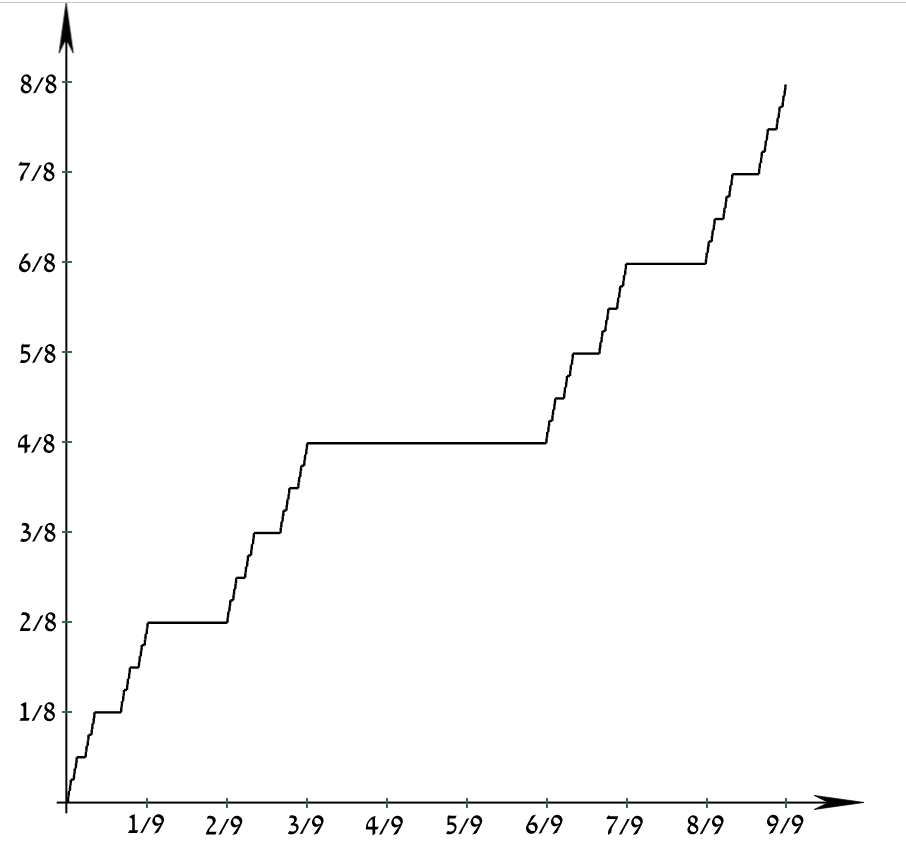
\includegraphics
        [width=\linewidth,height=0.2\textheight]{png/CantorFunc.png}
        \caption{Cantor function, download from Wikipedia.}
    \end{figure}
\end{defn}
\begin{exc}
    Let $f:[0,1]\rightarrow[0,1]$ be the Cantor function, 
    and let $g(x)=f(x)+x$.
    \begin{enumerate}
        \item $g$ is a bijection from $[0,1]$ to $[0,2]$, 
        and $h=g^{-1}$ is continuous from $[0,2]$ to $[0,1]$.
        \item If $C$ is a Cantor set, $m(g(C))=1$.
        \item $g(C)$ contains a Lebesgue nonmeasurable set $A$. 
        Let $B=g^{-1}(A)$, $B$ is Lebesgue measurable but not Borel.
        \item There exist a Lebesgue measurable function $F$ and a 
        continuous function $G$ on $\mathbb{R}$ such that 
        $F\circ G$ is not Lebesgue measurable.
    \end{enumerate}
\end{exc}
\begin{proof}
    (1)$f(x)$ is monotone increasing, and naturally $p(x)=x$
    is a strictly increasing function, and hence $g(x)=f(x)+x$
    x is also strictly increasing and therefore injective. 
    Next, to show surjectivity, note that $g$ is a continuous function, 
    and $g(0)=0$, $g(1)=2$; hence, by the intermediate value theorem, 
    $g$ is surjective. We now have all the necessary components to 
    conclude that $g$ is a bijection, and since $g$ is a
    continuous bijective function, and $[0,1]$ is compact, 
    $g^{-1}$ is continuous from $[0,2]$ to $[0,1]$.

    (2)Firstly, by $g$'s surjectivity, and $C$ being measurable, 
    we see that:
    \begin{displaymath}
        \begin{array}{rl}
            g([0,1]\setminus C)\cup g(C)=g([0,1]\cap C^c)\cup g(C)=[0,2]\\
            \Rightarrow m(g(C))+m(g([0,1]\setminus C))=2.
        \end{array}
    \end{displaymath}
    Next, since $C$ is a closed set $\Rightarrow$ $[0,1]\setminus C$
    is open set. Therefore, since all open subsets of $[0,1]$ may
    be written as a countable union of disjoint open sets, 
    let us write $[0,1]\setminus C=\cup_{1}^{\infty}O_j$, $O_j=(a_j,b_j)$.
    Now, since $f$ is by construction constant on $[0,1]\setminus C$,
    and $m(C)=0\Rightarrow m([0,1]\setminus C)=1\Rightarrow
    m(\cup_{1}^{\infty}O_j)=1$.
    \begin{displaymath}
        \begin{array}{rl}
            m(g([0,1]\setminus C))&=m(g(\cup_{1}^{\infty}O_j))
            =\sum_{1}^{\infty}m(g(O_j))\\
            &=\sum_{1}^{\infty}(m(f(b_j)-f(a_j))+m(b_j-a_j))\\
            &=\sum_{1}^{\infty}m(O_j)\\
            &=m(\cup_{1}^{\infty}O_j)\\
            &=1
        \end{array}
    \end{displaymath}  
    And hence $m(g(C))=1$.
    
    (3)To show Lebesgue measurability, naturally $B\subset C$,
    and since $C$ is measurable with measure $m(C)=0$, it implies
    $m(B)\leq m(C)=0$, and hence Lebesgue measurable since null 
    sets are measurable. For the sake of contradiction, suppose
    $B=g^{-1}(A)$ is Borel measurable. In part (1), we showed that
    $g^{-1}$ is continuous and bijective; therefore 
    $g(B)=g(g^{-1}(A))=A$. However, by the continuity of $g$,
    if $g^{-1}(A)$ was Borel, so too would $g(g^{-1}(A))=A$,
    hence a contradiction since $A$ is not Lebesgue
    measurable; therefore, $B$ cannot be Borel measurable.

    (4)Let $F=\chi_{B}$;
    \begin{equation}
        F(x)=\left\{
            \begin{array}{rl}
                1, &x\in B, \\
                0, &x\notin B,
            \end{array}
        \right.
    \end{equation}
    And also set $G=g^{-1}$. Naturally $G$ is Lebesgue measurable 
    since it is continuous, we now wish to prove that so too is $F$. 
    This can be seen by noticing $F^{-1}((a,\infty))=\emptyset$ or $B$
    or $\mathbb{R}$, , but all these possibilities are Lebesgue measurable,
    hence $F$ is Lebesgue measurable. We can now look at the following 
    reasoning:
    \begin{displaymath}
        \begin{array}{rl}
            (F\circ G)^{-1}([\frac{1}{2},\infty))&=G^{-1}\circ F^{-1}([\frac{1}{2},\infty))\\
            &=\{x\in[0,2]|\chi_B(g^{-1}(x))\in[\frac{1}{2},\infty)\} \\
            &=\{x\in[0,2]|g^{-1}(x)\in B\} \\
            &=G^{-1}(B)=g(g^{-1}(B))=A,
        \end{array}
    \end{displaymath}
    Now since $A$ is not Lebesgue measurable, 
    $F\circ G$ also will not be Lebesgue measurable.
\end{proof}
\begin{prop}
    \label{Prop:ComplexMeasurableFunc}
    $f:X\rightarrow\mathbb{C}$ is $\M$-measurable iff $\text{Re}f$, 
    $\text{Im}f$ are $\M$-measurable. 
\end{prop}
\begin{proof}
    Choose $\pi_{1}(z):=\text{Re}z$, $\pi_{2}(z):=\text{Im}z$, 
    then $\pi_{1},\pi_{2}$ are both measurable. If $f$ is 
    $\M$-measurable, 
    then $\text{Re}f=\pi_{1}\circ f$, $\text{Im}f=\pi_{2}\circ f$ 
    are both $\M$-measurable.

    If $\text{Im}f$, $\text{Re}f$ are both measurable, i.e. 
    $\pi_1\circ f$, $\pi_{2}\circ f$ are measurable, then for 
    any Borel set $\mathcal{B}\subset\mathbb{R}$, 
    $f^{-1}(\pi_{\alpha}^{-1}(\mathcal{B}))\in\M$ for 
    $\alpha=1,2$. $f$ is measurable 
    follows from $\mathcal{B}_{\mathbb{C}}
    =\mathcal{B}_{\mathbb{R}}\otimes
    \mathcal{B}_{\mathbb{R}}$ and 
    Proposition \ref{Prop:DescribeMeasFunc}.
\end{proof}
\begin{prop}
    \label{Prop:MeasFuncLinear}
    If $f,g:X\rightarrow\mathbb{C}$ are 
    $\M$-measurable, so are $f+g$, $fg$. 
\end{prop}
\begin{proof}
    Define $F:X\rightarrow \mathbb{C}\times\mathbb{C}$, 
    $F(x):=(f(x),g(x))$, 
    $\phi,\psi:\mathbb{C}\times\mathbb{C}\rightarrow\mathbb{C}$ 
    are 
    \begin{displaymath}
        \phi(z,w):=z+w,\quad \psi(z,w):=zw,
    \end{displaymath}
    then $F$ is 
    $(\M,\mathcal{B}_{\mathbb{C}\times\mathbb{C}})$-measurable, 
    $\phi,\psi$ are 
    $(\mathcal{B}_{\mathbb{C}\times\mathbb{C}},
    \mathcal{B}_{\mathbb{C}})$-measurable. So are 
    $f+g=\phi\circ F$, $fg=\psi\circ F$.
\end{proof}
\begin{rem}
    Proposition \ref{Prop:MeasFuncLinear} shows that 
    all the $\M$-measurable functions form an algebra.
\end{rem}
\begin{ntn}
    The \textit{generalized real line} 
    is denoted by:
    \begin{displaymath}
        \bar{\mathbb{R}}:=[-\infty,\infty]
        =\mathbb{R}\cup\{-\infty,\infty\}.
    \end{displaymath}
\end{ntn}
\begin{prop}
    \label{Prop:LimitProperties}
    $\forall j\in\mathbb{N}$, 
    $f_{j}:X\rightarrow\bar{\mathbb{R}}$ are 
    measurable functions, then 
    $g_{1}(x):=\limsup_{j\rightarrow\infty}f_{j}(x)$, 
    $g_{2}(x):=\liminf_{j\rightarrow\infty}f_{j}(x)$ 
    are measurable.
\end{prop}
\begin{exc}
    Prove Proposition \ref{Prop:LimitProperties}.
\end{exc}
\begin{proof}
    Set $m(x)=\sup_{j}f_{j}(x)$, $n(x)=\inf_{j}f_{j}(x)$.
    By the truth that $f_{j}:X\rightarrow\bar{\mathbb{R}}$ are 
    measurable functions, $m^{-1}((a,\infty])=
    \cup_{1}^{\infty}f_{j}^{-1}((a,\infty])$,  $n^{-1}([\infty,a))=
    \cup_{1}^{\infty}f_{j}^{-1}([\infty,a))$, so $m(x)$, $n(x)$
    are measurable. More generally, if $h_k(x)=\sup_{j>k}f_j(x)$
    then $h_k$ is measurable for each $k$, so $g_1(x)=\inf_{k}h_k(x)$
    is measurable, and likewise for $g_2(x)$.
\end{proof}
\begin{defn}
    Given $f:X\rightarrow\bar{\mathbb{R}}$, 
    the \textit{positive part }of $f$ is:
    \begin{displaymath}
        f^{+}(x):=\max(f(x),0),
    \end{displaymath}
    and the \textit{negative part }of $f$ 
    is:
    \begin{displaymath}
        f^{-}(x):=\max(-f(x),0).
    \end{displaymath}
\end{defn}
\begin{rem}
    If $f$ is measurable, so are $f^{+}$ and 
    $f^{-}$.
\end{rem}
\begin{defn}
    Given $f:X\rightarrow\mathbb{C}$, the 
    \textit{polar decomposition }of $f$ is 
    $f:=(\sgn f)|f|$ where 
    \begin{displaymath}
        \sgn(z)=\left\{
            \begin{array}{rl}
                \frac{z}{|z|},z\neq 0;
                0,z=0.
            \end{array}
        \right.
    \end{displaymath}
\end{defn}
\begin{rem}
    If $f$ is measurable, so are $\sgn f$ and $|f|$.
\end{rem}
\begin{defn}
    \label{Defn:CharFunc}
    For $E\subset X$, the \textit{characteristic function} of $X$ 
    is given by $\chi_{E}(x)$ with:
    \begin{displaymath}
        \chi_{E}(x):=\left\{
            \begin{array}{rl}
                1,x\in E;\\
                0,x\notin E.\\
            \end{array}
        \right.
    \end{displaymath}
\end{defn}
\begin{defn}
    \label{Defn:SimpleFunc}
    A \textit{simple function }on $X$ is given by 
    $f:X\rightarrow\mathbb{C}$ with 
    $f(x)=\sm{j}{n}z_{j}\chi_{E_{j}}$, where $E_j\in\M$, 
    $z_j\in\mathbb{C}$, satisfies $\forall j\neq k$ $z_{j}\neq z_{k}$, 
    $E_j\cap E_k=\emptyset$.
\end{defn}
\begin{thm}
    \label{Thm:ApproxMeasFuncBySimpleFunc}
    If $f:X\rightarrow[0,\infty]$ is measurable, 
    then there exists simple functions $\{\phi_{n}\}$ such that 
    $0\le\phi_{1}\le\ldots\le\phi_{n}\le\ldots\le f$, 
    $\phi_{n}\rightarrow f$ pointwise, and 
    $\phi_{n}\rightarrow f$ uniformly in any set 
    where $f$ is bounded.
\end{thm}
\begin{exc}
    For $0\le k\le 2^{2n}-1$, mark 
    \begin{displaymath}
    E_{n}^{k}:=f^{-1}((k2^{-n},(k+1)2^{-n}]),\quad 
    F_{n}:=f^{-1}((2^{n},\infty]),
    \end{displaymath}
    then define 
    \begin{displaymath}
        \phi_{n}:=\sum_{k=0}^{2^{2n}-1}k2^{-n}\chi_{E_{n}^{k}}
        +2^{n}\chi_{F_{n}},
    \end{displaymath}
    show $\{\phi_{n}\}$ satisfies the condition of 
    Theorem \ref{Thm:ApproxMeasFuncBySimpleFunc}.
\end{exc}
\begin{proof}
    By the truth that $\chi_{E}(x)\geq 0$, it is easily checked
    that $\phi_{n}\leq\phi_{n+1}$ for all $n$, and 
    $0\leq f-\phi_{n}\leq 2^{-n}$ on the set where 
    $f\leq 2^{-n}$. The result therefore follows.
\end{proof}
\section{Integration}
\begin{defn}
    \label{Defn:IntegralOfSimpleFunc}
    Given a measurable space $(X,\M,\mu)$, define 
    \begin{displaymath}
        \mathcal{L}^{+}:=\{\text{measurable functions }f:
        X\rightarrow[0,\infty]\},
    \end{displaymath}
    if $\phi\in \mathcal{L}^{+}$ is a simple function with 
    $\phi=\sm{i}{n}\phi_{i}\chi_{E_i}$, then 
    the \textit{integration of $\phi$} is 
    \begin{displaymath}
        \int\phi\dif\mu:=\sm{i}{n}\phi_{i}\mu(E_i).
    \end{displaymath}
\end{defn}
\begin{rem}
    We mark $0\cdot\infty=0$.
\end{rem}
\begin{prop}
    \label{Prop:PropertyOfSimpleInt}
    For simple functions $\phi$, $\psi\in\mathcal{L}^{+}$. 
    \begin{enumerate}
        \item If $c\ge 0$, then $\int c\phi=c\int\phi$. 
        \item $\int(\phi+\psi)=\int\phi+\int\psi$.
        \item If $\phi\le\psi$, then $\int\phi\le\int\psi$. 
        \item $A\mapsto \int_{A}\phi\dif\mu$ is a measure on $\M$.
    \end{enumerate}
\end{prop}
\begin{exc}
    Prove Proposition \ref{Prop:PropertyOfSimpleInt}.
\end{exc}
\begin{proof}
    (a) id trivial. For (b), let $\sum_{1}^{n}a_j\chi_{E_j}$ and 
    $\sum_{1}^{m}b_k\chi_{F_k}$ be the standard representation of 
    $\phi$ and $\psi$. Then $E_j=\cup_{k=1}^{m}(E_j\cap F_k)$ and
    $F_k=\cup_{j=1}^{n}(E_j\cap F_k)$ since $\cup_{1}^{n}E_j=
    \cup_{1}^{m}F_k=X$, and these unions are disjoint. Hence the
    finite additivity of $\mu$ implies that
    \begin{displaymath}
        \int\phi+\int\psi=\sum_{j,k}(a_j+b_k)\mu(E_j\cap F_k),
    \end{displaymath}
    and the same reasoning show that the sum on the right equals
    $\int(\phi+\psi)$. Moreover, if $\phi\leq\psi$, then $a_j\leq b_k$
    whenever $E_j\cap F_k\neq\emptyset$, so
    \begin{displaymath}
        \int\phi=\sum_{j,k}a_j\mu(E_j\cap F_k)\leq\sum_{j,k}b_k\mu(E_j\cap F_k)
        =\int\psi,
    \end{displaymath}
    which proves (c). Finally, if $\{A_k\}$ is a disjoint sequence in $\mathcal{M}$
    and $A=\cup_{1}^{\infty}A_k$,
    \begin{displaymath}
        \int_A\phi=\sum_ja_j\mu(A\cap E_j)=\sum_{j,k}a_j\mu(A_k\cap E_j)
        =\sum_k\int_{A_k}\phi,
    \end{displaymath}
    which establishes (d).
\end{proof}
\begin{defn}
    \label{Defn:IntegralForPositive}
    For $f\in \mathcal{L}^{+}$, define 
    \begin{displaymath}
        \int f\dif\mu:=\sup\left\{\int\phi\dif\mu:0\le\phi\le f,
        \;\phi\text{ is simple}\right\}.
    \end{displaymath}
\end{defn}
\begin{rem}
    Definition \ref{Defn:IntegralForPositive} is straightforward 
    from Theorem \ref{Thm:ApproxMeasFuncBySimpleFunc}.
\end{rem}
\begin{defn}
    \label{Defn:RealValuedFuncInt}
    If $f:X\rightarrow\bar{\mathbb{R}}$, we say 
    $f$ is \textit{integrable} iff $\int|f|\dif\mu<\infty$, 
    then 
    \begin{displaymath}
        \int f\dif\mu:=\int f^{+}\dif\mu-\int f^{-}\dif\mu.
    \end{displaymath}
\end{defn}
\begin{defn}
    \label{Defn:ComplexValuedFuncInt}
    If $f:X\rightarrow\mathbb{C}$, we say $f$ is \textit{integrable} 
    iff $\int|f|\dif\mu<\infty$, then 
    \begin{displaymath}
        \int f\dif\mu=\int \text{Re}f\dif\mu+i\int\text{Im}f\dif\mu.
    \end{displaymath}
\end{defn}
\begin{exc}
    Show that all the integrable 
    functions on $X$ forms a vector space.
\end{exc}
\begin{proof}
    We only need to prove that all the integrable 
    functions on $X$ satisfy their closure under addition
    and their closure under scalar multiplication. 
    $\forall \lambda\in\mathbb{C}$ and if $f$ 
    is \textit{integrable}, then 
    $\int|\lambda f|d\mu=|\lambda|\int|f|d\mu<\infty$,
    so $\lambda f$ is \textit{integrable}.
    If $f$ and $g$ is \textit{integrable},
    $\int|f+g|d\mu\leq\int|f|d\mu+\int|g|d\mu<\infty$,
    so $f+g$ is \textit{integrable}.
\end{proof}
\begin{ntn}
    If the measure $\mu$ is clear, 
    we write $\int\phi$ to 
\end{ntn}
\begin{thm}[Monotone Convergence Theorem]
    \label{Thm:MCT}
    If $\{f_{n}\}\subset\mathcal{L}^{+}$ such that 
    $\forall j\in\mathbb{N}$, $f_j\le f_{j+1}$, and 
    $f=\lim_{n\rightarrow\infty}f_{n}$, then 
    $\int f=\lim_{n\rightarrow\infty}\int f_n$.
\end{thm}
\begin{proof}
    We divide this proof into 3 steps. 

    First, since $\forall x\in X$, $\{f_{n}(x)\}$ is an increasing 
    sequence on $[0,\infty]$, $f(x):=\lim_{n\rightarrow\infty}f_{n}(x)$ 
    exists in $[0,\infty]$ as well, and $\forall n\in\mathbb{N}$, 
    $f_{n}(x)\le f(x)$.

    Second, $\forall n\in\mathbb{N}$, $f_{n}\le f$ means 
    \begin{displaymath}
        \forall n\in\mathbb{N}, \int f_{n}\le\int f,
    \end{displaymath}
    choose $n\rightarrow\infty$, 
    it shows $\lim_{n\rightarrow\infty}f_{n}\le\int f$.

    Third, given $\alpha\in(0,1)$ and simple function $\phi$ 
    such that $0\le\phi\le f$, let 
    \begin{displaymath}
        E_n:=\{x:f_{n}(x)\ge\alpha\phi(x)\},
    \end{displaymath}
    then $E_{n}$ is increasing, and $\cp{n}{\infty}E_n=X$, thus:
    \begin{displaymath}
        \forall\alpha\in(0,1),\;
        \int f_n\ge\int_{E_n}f_{n}\ge\alpha\int_{E_n}\phi.
    \end{displaymath}
    Set $n\rightarrow\infty$, it yields $\forall\alpha\in(0,1)$, 
    \begin{displaymath}
        \lim_{n\rightarrow\infty}\int f_n\ge\alpha\int\phi.
    \end{displaymath}
    So $\lim_{n\rightarrow\infty}\int f_n\ge\int\phi$. 
    Choose supermum, it means 
    $\lim_{n\rightarrow\infty}f_n\ge\int f$. 
    It completes the proof.
\end{proof}
\begin{exc}
    In the proof of Theorem \ref{Thm:MCT}, 
    can we replace $\alpha\phi$ by $\phi-\epsilon$? 
    Why?
\end{exc}
\begin{proof}
    No! It may make $\phi-\epsilon\leq0$ in some measurable
    sets $E_j$.
\end{proof}
\begin{thm}
    \label{Thm:SeriesAndInt}
    For $\{f_n\}\subset \mathcal{L}^{+}$, 
    $f:=\sm{n}{\infty}f_n$, 
    $\int f=\sm{n}{\infty}\int f_n$.
\end{thm}
\begin{exc}
    Prove Theorem \ref{Thm:SeriesAndInt}.
\end{exc}
\begin{proof}
    Let $\phi_n=\sum_{1}^{n}f_n$, since 
    $\{f_n\}\subset\mathcal{L}^{+}$, 
    $\{\phi\}\subset\mathcal{L}^{+}$, such that 
    $\forall j\in\mathbb{N}$, $\phi_j\leq\phi_{j+1}$, and
    $f=\lim_{n\rightarrow\infty}\phi_n$,
    then by Theorem \ref{Thm:MCT} $\int f=\lim_{n\rightarrow\infty}\int\phi_n
    =\lim_{n\rightarrow\infty}\int\sum_{1}^{n}f_n
    =\sum_{1}^{\infty}\int f_n$.
\end{proof}
\begin{rem}
    Theorem \ref{Thm:SeriesAndInt} shows that 
    term-by-term integration property holds 
    for positive functions.
\end{rem}
\begin{prop}
    \label{Prop:PositiveIntZero}
    If $f\in \mathcal{L}^{+}$, then 
    $\int f=0\Leftrightarrow f=0$ a.e..
\end{prop}
\begin{proof}
    We divide this proof into three steps. 

    First, if $f$ is a simple function, i.e. 
    $f=\sm{i}{n}a_{i}\chi_{E_i}$, then 
    \begin{displaymath}
        \int f=0\Leftrightarrow
        \sm{i}{n}a_{i}\mu(E_i)=0.
    \end{displaymath}
    Since $a_{i}\ge 0$, if $a_{i_{0}}>0$, 
    it means 
    \begin{displaymath}
        \sm{i}{n}a_{i}\mu(E_i)
        \ge a_{i_0}\mu(E_{i_0})=0,
    \end{displaymath}
    i.e. $\mu(E_{i_0})=0$, it means $f=0$ a.e..
    If for a simple function $f$, $f=0$ a.e., it's clear that 
    $\int f=0$.

    Second, for $f\in \mathcal{L}^{+}$, if $f=0$ a.e., 
    $\forall$ simple function $0\le\phi\le f$, 
    $\phi=0$ a.e., so $\int\phi=0$, which means $\int f=0$.

    Finally, if $\int f=0$, let $E_{n}:=\{x:f(x)>\frac{1}{n}\}$, 
    then $\cp{n}{\infty}E_{n}=\{x:f(x)\neq 0\}$. 
    Assume $f=0$ a.e. isn't true, it means $\exists E_{n}$ 
    such that $\mu(E_n)>0$. 
    But 
    \begin{displaymath}
        \int f\ge\int_{E_n}f\ge\frac{1}{n}\int_{E_n}1
        =\frac{1}{n}\mu(E_n)>0,
    \end{displaymath}
    contradict! So $f=0$ a.e..
\end{proof}
\begin{coro}
    For $\{f_{n}\}\subset\mathcal{L}^{+}$, 
    $f\in\mathcal{L}^{+}$, 
    assume for a.e. $x\in X$, $\{f_{n}(x)\}$ is increasing and 
    $\lim_{n\rightarrow\infty}f_{n}(x)=f(x)$, 
    then 
    \begin{displaymath}
        \int f=\lim_{n\rightarrow\infty}\int f_n.
    \end{displaymath}
\end{coro}
\begin{thm}[Fatou's Lemma]
    \label{Thm:Fatou}
    For $\{f_{n}\}\subset\mathcal{L}^{+}$, 
    \begin{displaymath}
        \int\liminf_{n\rightarrow\infty}f_n\le\liminf_{n\rightarrow\infty}
        \int f_n.
    \end{displaymath}
\end{thm}
\begin{proof}
    $\forall k\ge 1$, $j\ge k$, $\inf_{n\ge k}f_n\le f_{j}$, 
    thus 
    \begin{displaymath}
        \forall j\ge k,\;
        \int\inf_{n\ge k}f_n\le\int f_{j}.
    \end{displaymath} 
    So 
    \begin{displaymath}
        \int\inf_{n\ge k}f_n\le\inf_{j\ge k}\int f_{j}.
    \end{displaymath}
    Then, since $g_{k}:=\inf_{n\ge k}f_{n}$ is increasing, 
    by Theorem \ref{Thm:MCT}, 
    \begin{displaymath}
        \begin{array}{rl}
        \int\liminf_{n\rightarrow\infty}f_{n}
        &=\int\lim_{k\rightarrow\infty}\inf_{n\ge k}f_{n}\\
        &=\lim_{k\rightarrow\infty}\int\inf_{n\ge k}f_{n}\\
        &\le\lim_{k\rightarrow\infty}\inf_{n\ge k}\int f_{n}\\
        &=\liminf_{n\rightarrow\infty}\int f_{n}.
        \end{array}
    \end{displaymath}
\end{proof}
\begin{exc}
    Give a sequence $\{f_{n}\}\subset\mathcal{L}^{+}$, 
    such that 
    \begin{displaymath}
        \int\liminf_{n\rightarrow\infty}f_{n}<
        \liminf_{n\rightarrow\infty}\int f_{n}.
    \end{displaymath}
\end{exc}
\begin{proof}
    We can consider function
    \begin{displaymath}
        f_n(x)=
        \left\{\begin{array}{rl}
            &n \quad \textit{for} \quad x\in(0,\frac{1}{n}),\\
            &0 \quad \textit{otherwise}\\
        \end{array}
        \right.
    \end{displaymath}
    These sequences converge pointwise (respectively uniformly) 
    to the zero function (with integral equal to zero), 
    yet each sequence has an integral of one.
\end{proof}
\begin{prop}
    \label{Prop:PropOfL1}
    \begin{enumerate}
        \item $f$ is integrable on $X$ 
        means $\{x:f(x)\neq 0\}$ is $\sigma$-finite. 
        \item If $f,g$ are integrable, then TFAE:
        \begin{enumerate}
            \item $\forall E\in\M$, $\int_{E}f=\int_{E}g$.
            \item $\int|f-g|=0$.
            \item $f=g$ a.e..
        \end{enumerate}
    \end{enumerate}
\end{prop}
\begin{proof}
    (1). If $f\in\mathcal{L}^{+}$, 
    $\forall n\in\mathbb{N}^{+}$, since $f$ is integrable, 
    $\mu(\{x:f(x)>\frac{1}{n}\})<\infty$. So $\{f>0\}$ is $\sigma$-finite. 
    If $f\in L^{1}$, then 
    \begin{displaymath}
        \{x:f(x)\neq 0\}=\{\text{Re}f\neq 0\}\cup\{\text{Im}f\neq 0\}
    \end{displaymath}
    is $\sigma$-finite. It completes the proof. 

    (2). $(b)\Leftrightarrow (c)$: Follows from Proposition 
    \ref{Prop:PositiveIntZero}.

    $(b)\Rightarrow (a)$: Since $\int|f-g|=0$, 
    \begin{displaymath}
        \begin{array}{rl}
        \left|\int_{E}f-\int_{E}g\right|
        &=\left|\int\chi_{E}(f-g)\right|\\
        &\le\int\left|\chi_{E}(f-g)\right|\\
        &\le\int|f-g|=0.\\
        \end{array}
    \end{displaymath}
    So $\int_{E}f=\int_{E}g$. 

    $(a)\Rightarrow (c)$: If $\mu(\{f\neq g\})\neq 0$, 
    choose $u:=\text{Re}(f-g)$, $v:=\text{Im}(f-g)$, 
    one of $u^{\pm},v^{\pm}$ is nonzero on some $E$ such that $\mu(E)>0$. 
    WLOG, say $E=\{u^{+}>0\}$, then 
    \begin{displaymath}
        \text{Re}\left(\int_{E}f-\int_{E}g\right)=\int_{E}u^{+}>0,
    \end{displaymath}
    contradict!
\end{proof}
\begin{rem}
    In Proposition \ref{Prop:PropOfL1}, it's clear that if $f=g$ a.e., 
    then $f$ is equivalent to $g$ by integral.
\end{rem}
\begin{defn}
    \label{Defn:L1space}
    $L^{1}(X,\mu)$ is the set of equivalent classes of 
    a.e. defined integrable functions 
    on $X$, where $f\sim g$ iff $f=g$ a.e..
\end{defn}
\begin{thm}[Dominated Convergence Theorem]
    Assume there exists a sequence $\{f_{n}\}$ such that 
    \begin{itemize}
        \item $f_{n}\rightarrow f$ a.e.,
        \item There exists $g\in L^{1}(X,\mu)$ such that 
        $|f_n|\le g$ a.e.,
    \end{itemize}
    then $f\in L^{1}(X,\mu)$ and 
    $\int f=\lim_{n\rightarrow\infty}\int f_{n}$.
\end{thm}
\begin{proof}
    WLOG, we assume $f,f_{n}:X\rightarrow \mathbb{R}$, 
    then $g+f_n\ge 0$ a.e. and $g-f_n\ge 0$ a.e.. 
    By Fatou's Lemma:
    \begin{displaymath}
        \left\{
            \begin{array}{rl}
                \int (g+f)&\le\liminf_{n\rightarrow\infty}\int(g+f_n),\\
                \int (g-f)&\le\liminf_{n\rightarrow\infty}\int(g-f_{n}),
            \end{array}
        \right.
    \end{displaymath}
    so $\limsup_{n\rightarrow\infty}\int f_{n}\le\int f
    \le\liminf_{n\rightarrow\infty}\int f_{n}$, which means 
    $\int f=\lim_{n\rightarrow\infty}\int f_n$.
\end{proof}
\begin{coro}
    \label{Cor:AbsoluteConvergence}
    If $\{f_{j}\}\subset L^{1}(X,\mu)$ and 
    $\sm{i}{\infty}\int|f_i|<\infty$, then 
    $\sm{i}{\infty}f_{i}$ converges a.e. to some $f\in L^{1}(X,\mu)$ 
    and $\int f=\sm{i}{\infty}\int f_{i}$.
\end{coro}
\begin{exc}
    Show that if $\sm{i}{\infty}|a_{i}|<\infty$ then 
    $\sm{i}{\infty}a_{i}$ converges 
    by Corollary \ref{Cor:AbsoluteConvergence}.
\end{exc}
\begin{proof}
    Suppose that $\{f_j\}\subset L^{1}(X,\mu)$ such that $\int|f_j|=|a_j|$
    and $\sm{i}{\infty}|f_i|=\sm{i}{\infty}|a_{i}|<\infty$, so function
    $g=\sm{i}{\infty}|f_i|\in L^{1}(X,\mu)$. In particular, by Corollary
    \ref{Cor:AbsoluteConvergence}, the series $\sm{i}{\infty}f_j$ converges,
    so $\sm{i}{\infty}a_{i}$ converges.
\end{proof}
\begin{exc}
    Show that simple functions are 
    dense in $L^{1}(X,\mu)$.
\end{exc}
\begin{proof}
    By Theorem \ref{Thm:ApproxMeasFuncBySimpleFunc}, we can choose
    $\{\phi_n\}$, the $\int|\phi_n-f|<\epsilon$ for $n$ sufficiently
    large by the dominated convergence theorem, since $|\phi_n-f|\leq2|f|$.
\end{proof}
\begin{thm}
    \label{Thm:ChangeOrder}
    $f:X\times[a,b]\rightarrow\mathbb{C}$, and 
    $\forall t_{0}\in[a,b]$, $h(x):=f(x,t_0)\in L^{1}(X,\mu)$, 
    let $F(t):=\int f(x,t)\dif\mu(x)$,
    \begin{enumerate}
        \item Suppose $\exists g\in L^{1}(X,\mu)$ such that 
        $\forall x,t$, $|f(x,t)|\le g(x)$, if 
        $\forall x\in X$, $\lim_{t\rightarrow t_{0}}f(x,t)=f(x,t_0)$, 
        then $\lim_{t\rightarrow t_{0}}F(t)=F(t_0)$.
        \item Suppose $\pdfFrac{f}{t}$ exists, and 
        $\exists g\in L^{1}(X,\mu)$ such that 
        $\left|\pdfFrac{f}{t}(x,t)\right|\le g(x)$, then 
        $F$ is differentiable and 
        $F'(t)=\int\pdfFrac{f}{t}(x,t)\dif\mu(x)$.
    \end{enumerate}
\end{thm}
\begin{proof}
    $(1)$ Take a sequence $\{t_{n}\}\subset[a,b]\setminus\{t_0\}$ 
    with $t_{n}\rightarrow t_0$, and set $f_{n}(x):=f(x,t_{n})$, 
    then $\lim_{n\rightarrow\infty}f_{n}(x)=f(x,t_{0})$. 
    Since $\forall n$, $|f_{n}|\le g$, by DCT:
    \begin{displaymath}
        \begin{array}{rl}
        F(t_0)
        &=\int f(x,t_{0})=\int\lim_{n\rightarrow\infty}f_{n}(x)\\
        &=\lim_{n\rightarrow\infty}\int f_{n}(x)
        =\lim_{n\rightarrow\infty}F(t_{n}).\\
        \end{array}
    \end{displaymath}

    $(2)$ Mark 
    \begin{displaymath}
        h_{n}(x):=\frac{f(x,t_n)-f(x,t_0)}{t_n-t_0},
    \end{displaymath}
    then 
    \begin{displaymath}
        \pdfFrac{f}{t}(x,t_0)=\lim_{n\rightarrow\infty}h_{n}(x).
    \end{displaymath}
    By Lagrangian Mean Value Theorem, 
    \begin{displaymath}
        |h_{n}(x)|\le\sup_{t\in[a,b]}
        \left|\pdfFrac{f}{t}(x,t)\right|\le g(x),
    \end{displaymath}
    then by DCT: 
    \begin{displaymath}
        \begin{array}{rl}
        F'(t_0)&=\lim_{n\rightarrow\infty}\frac{F(t_n)-F(t_0)}{t_n-t_0}
        =\lim_{n\rightarrow\infty}\int h_n(x)\\
        &=\int\lim_{n\rightarrow\infty}h_{n}(x)
        =\int\pdfFrac{f}{t}(x,t_0)\dif\mu(x).
        \end{array}
    \end{displaymath}
\end{proof}
\begin{rem}
    Theorem \ref{Thm:ChangeOrder} 
    explains when the order of integration and limits can be exchanged.
\end{rem}
\begin{thm}
    \label{Thm:RiemannIntegrable}
    Given a bounded function $f:[a,b]\rightarrow\mathbb{R}$, 
    $E:=\{x:\text{ }f\text{ is discontinuous at }x\}$,
    then $f$ is Riemann integrable iff $m(E)=0$. 
\end{thm}
\begin{exc}
    Prove Theorem \ref{Thm:RiemannIntegrable}.
\end{exc}
\begin{proof}
    Set $H(x)=\lim_{\delta\rightarrow0}\sup_{|y-x|<\delta}f(y)$ and
    $h(x)=\lim_{\delta\rightarrow0}\inf_{|y-x|<\delta}f(y)$.
    If $H(x)=h(x)$, $H(x)=h(x)=\lim_{y\rightarrow x}f(y)$ exists.
    Since $h(x)\leq f(x)\leq H(x)$ is true, we have 
    $\lim_{y\rightarrow x}f(y)=f(x)$. Thus, $f$ is continuous at $x$.
    Conversely, if $f$ is continuous at $x$, 
    $\lim_{y\rightarrow x}f(y)$ exists, so $H(x)=h(x)=\lim_{y\rightarrow x}f(y)$.
    
    Let $\{P_n\}$ be a sequence of partitions of $[a, b]$, $\forall x\in\mathbb{R}$,
    let $\delta>0$ 0 be arbitrary real number such that 
    $[x-\delta,x+\delta]\subset(t_{k-1},t_k]$, where $(t_{k-1},t_k]$
    is a partition of $P_n$. Then we can always choose a partition
    \begin{displaymath}
        P_s=\{a=s_0<s_1<\ldots<s_{J_s}=b\},
    \end{displaymath}
    such that $x\in(s_{k-1},s_k]$ and
    \begin{displaymath}
        (s_{k-1},s_k]\subset[x-\delta,x+\delta]\subset(t_{k-1},t_k],
    \end{displaymath}
    where $s>n$. Thus $M_k^s=G_{P_s}\leq\sup_{|y-x|<\delta}f(y)\leq
    G_{P_n}=M_k^n$, and $m_k^n=g_{P_n}\leq\inf_{|y-x|<\delta}f(y)\leq
    g_{P_s}=M_k^s$, since $s\rightarrow\infty$ and $\delta\rightarrow0$ 
    if $n\rightarrow\infty$,  $H(x)=\lim_{\delta\rightarrow0}
    \sup_{|y-x|<\delta}f(y)=G(x)$ and $h(x)=\lim_{\delta\rightarrow0}
    \inf_{|y-x|<\delta}f(y)=g(x)$, since $\{t_k\}$ is countable, 
    it is Lebesgue measure 0. So $G=H$ and $h=g$ a.e.

    Additionally, Note that $f$ is Riemann integrable iff $G = g$ 
    iff $H = h$ a.e. iff $f$ is continuous a.e. Thus, 
    $E:=\{x:\text{ }f\text{ is discontinuous at }x\}$,
    then $f$ is Riemann integrable iff $m(E)=0$.  
\end{proof}
\section{Convergence}
\begin{rem}
    In this section, we will introduce multiple modes of convergence, 
    and discuss their relationships.
\end{rem}
\begin{defn}
    \label{Defn:ConvergeInMeasure}
    For a sequence $\{f_{n}\}$ with $f_{n}:X\rightarrow\mathbb{C}$, 
    if $\forall\epsilon>0$, 
    \begin{displaymath}
        \lim_{n\rightarrow\infty}\mu(\{|f_n-f|>\epsilon\})=0,
    \end{displaymath}
    then $\{f_n\}$ \textit{converges to $f$ in measure.}
\end{defn}
\begin{defn}
    \label{Defn:CauchyInMeasure}
    If a sequence $\{f_{n}\}$ satisfies: $\forall\epsilon,\delta>0$, 
    $\exists N$, $\forall m,n\ge N$, 
    \begin{displaymath}
        \mu(|f_{m}-f_{n}|>\delta)<\epsilon,
    \end{displaymath}
    then $\{f_{n}\}$ is called a \textit{Cauchy sequence in measure}.
\end{defn}
\begin{exc}
    Show that $\{f_{n}\}$ be a Cauchy sequence in measure 
    is equivalent to the fact that 
    there exists $f:X\rightarrow\mathbb{C}$ such that 
    $f_{n}\rightarrow f$ in measure.
\end{exc}
\begin{proof}
    We can choose a subsequence $\{g_j\}=\{f_{n_j}\}$ of $\{f_n\}$
    such that if $E_j=\{x:|g_j-g_{j+1}|\geq2^{-j}\}$, then $\mu(E_j)
    \leq2^{-j}$. If $F_k=\cup_{j=k}^{\infty}E_j$, then $\mu(F_k)
    \leq\sum_{k}^{\infty}2^{-j}=2^{1-k}$, and if $x\notin F_k$, for
    $i\geq j\geq k$ we have $|g_j-g_i|\leq\sum_{l=j}^{i-1}|g_{l+1}-g_l|
    \leq\sum_{l=j}^{i-1}2^{-1}\leq2^{1-j}$. Thus $\{g_j\}$ is pointwise
    Cauchy on $F_k^c$. Let $F=\cap_{1}^{\infty}F_k=\lim\sup E_j$.
    Then $\mu(F)=0$, and if we set $f(x)=\lim g_j$ for $x\notin F$ 
    and $f(x)=0$ for $x\in F$, then $f$ is measurable and $g_j\rightarrow f$.
    Then $f_n\rightarrow f$ in measure, because $\{x:|f-g|\geq\epsilon\}
    \subset\{x:|f-f_n|\geq\frac{1}{2}\epsilon\}\cup
    \{x:|f_n-g|\geq\frac{1}{2}\epsilon\}$.
\end{proof}
\begin{defn}
    \label{Defn:ConvergenceInL1}
    For a sequence $\{f_n\}$, if 
    \begin{displaymath}
        \lim_{n\rightarrow\infty}\int|f_n-f|=0,
    \end{displaymath}
    we call $f_{n}$ \textit{converges to $f$ in $L^{1}$.}
\end{defn}
\begin{defn}
    \label{Defn:ConvergeAlmostEverywhere}
    For a sequence $\{f_n\}$, if for a.e. $x\in X$, 
    \begin{displaymath}
        \lim_{n\rightarrow\infty}f_{n}(x)=f(x),
    \end{displaymath}
    we call $f_{n}$ \textit{converges to $f$ a.e..}
\end{defn}
\begin{defn}
    \label{Defn:AlmostConvergesUniformly}
    For a sequence $\{f_n\}$, if there exists $\Sc\subset X$ 
    such that 
    $f_{n}\rightarrow f$ uniformly on $\Sc$, 
    and $\mu(X\setminus\Sc)=0$, 
    we call $f_{n}$ \textit{converges to $f$ almost uniformly}.
\end{defn}
\begin{exc}
    Find some examples $\{f_{n}\}$ such that: 
    \begin{itemize}
        \item $f_{n}$ converges to $f$ 
        almost uniformly but $f_{n}$ doesn't converge 
        to $f$ in $L^{1}$. 
        \item $f_{n}$ converges to $f$ in measure but 
        $f_{n}$ doesn't converge to $f$ in $L^{1}$.
        \item $f_{n}$ converges to $f$ in $L^{1}$ but 
        $f_{n}$ doesn't converge to $f$ a.e..
        \item $f_{n}$ converges to $f$ a.e. but 
        $f_{n}$ doesn't converge to $f$ in $L^{1}$.
    \end{itemize} 
\end{exc}
\begin{proof}
    (1)A classic example is the sequence of functions 
    $\{f_n(x)\}$ defined on the interval $[0, 1]$, 
    where $f_n(x) = n^2 \cdot x(1-x)^n$. This sequence 
    converges uniformly to 0, as for any $\varepsilon > 0$, we 
    can choose $N$ such that for $n > N$, $|f_n(x) - 0| = 
    |n^2 \cdot x(1-x)^n| < \varepsilon$ for all $x \in [0, 1]$.
    However, this sequence of functions does not converge in 
    $L^1$ to 0. We can compute:

    $$
    \begin{aligned}
    \int_{0}^{1} |f_n(x) - 0| \, dx & = \int_{0}^{1} n^2 \cdot x(1-x)^n \, dx \\
    & = \frac{n^2}{(n+1)(n+2)}
    \end{aligned}
    $$

    Therefore, $\lim_{n \to \infty} \int_{0}^{1} |f_n(x) - 0| \, 
    dx = \lim_{n^2 \to \infty} \frac{n}{(n+1)(n+2)} = 1 \neq 0$. 
    Hence, even though the sequence of functions converges uniformly 
    to 0, it does not converge in $L^1$ to 0.

    (2)A classic example is the sequence of functions $\{f_n(x)\}$ 
    defined on the unit interval $[0, 1]$, where $f_n(x) = n \cdot 
    \chi_{[0, \frac{1}{n}]}$. Here, $\chi_A$ denotes the indicator 
    function, which equals 1 if an element belongs to the set $A$, 
    and 0 otherwise.In this example, we observe that $f_n(x)$ converges 
    in measure to 0. This is because for any $\varepsilon > 0$, when 
    $n > \frac{1}{\varepsilon}$, $f_n(x)$ is almost everywhere 0. 
    That is, outside a set of measure 1, $f_n(x)$ is 0.
    However, we can compute the $L^1$ norm:

    $$
    \int_{0}^{1} |f_n(x) - 0| \, dx = \int_{0}^{1} n \cdot 
    \chi_{[0, \frac{1}{n}]} \, dx = 1
    $$

    Therefore, even though the sequence of functions converges in 
    measure to 0, it does not converge in $L^1$ to 0.

    (3)A classic example is the sequence of functions defined on the 
    interval $[0,1]$, given by $f_n(x) = x^n$. This function sequence 
    converges in the $L^1$ norm, as $\int_0^1 |x^n| dx = \frac{1}{n+1}$, 
    so $\lim_{n \to \infty} \int_0^1 |x^n| dx = 0$. However, this function 
    sequence does not converge almost everywhere on the interval $[0,1)$,
    as it does not converge at $x=1$.

    Thus, this example illustrates that a function sequence can converge in the $L^1$ norm 
    but not converge at certain points, and therefore, it is not almost everywhere convergent.
    
    (4)A classic example is the sequence of functions given by
    $f_n(x) = \frac{1}{n} \cdot \sin\left(\frac{x}{n}\right)$.
    This sequence of functions converges almost everywhere to zero, 
    as for any fixed $x$, as $n$ tends to infinity, $f_n(x)$ tends to zero.
    However, the sequence of functions does not converge in the $L^1$ 
    norm over the entire real line to zero.
    However,

    $$
    \begin{aligned}
    \|f_n\|_1 &= \int |n \cdot \sin\left(\frac{x}{n}\right)| \, dx \\
    &= \int | \sin(u) | \, du \quad (\text{let} u = \frac{x}{n}) \\
    &= 2,
    \end{aligned}
    $$

    Here, the integration is over the interval $[- \pi n, \pi n]$. 
    Therefore, the $L^1$ norm of $f_n(x)$ does not tend to zero as $n$ 
    tends to infinity.
\end{proof}
\begin{exc}
    Try to explain the convergence mode of random variable 
    sequence $\{X_{n}\}$ by the concepts above.
\end{exc}
\begin{proof}
    Random variable convergence in measure: Let $\{X_n\}$ and 
    $X$ be a sequence of random variables defined on the 
    probability space $(\Omega, \mathcal{F}, P)$. If for any 
    $\varepsilon > 0$, $\lim_{n \to \infty} P(\{|X_n - X| \geq 
    \varepsilon\}) = 0$, then the sequence of random variables 
    $\{X_n\}$ is said to converge in measure to $X$.

    Convergence almost everywhere: Let $\{X_n\}$ and $X$ be a 
    sequence of random variables defined on the probability space 
    $(\Omega, \mathcal{F}, P)$. If there exists an event $A$ with 
    probability 1, such that on the event $A$, $X_n$ converges to 
    $X$, then the sequence of random variables $\{X_n\}$ converges 
    almost everywhere to $X$.

    $L^1$ convergence: Let $\{X_n\}$ and $X$ be a sequence of random 
    variables defined on the probability space $(\Omega, \mathcal{F}, P)$.
    If $\lim_{n \to \infty} E[|X_n - X|] = 0$, then the sequence of 
    random variables $\{X_n\}$ converges in $L^1$ to $X$.
\end{proof}
\begin{rem}
    All convergence modes are not equivalent; 
    however, under certain conditions, 
    one mode of convergence may imply the other.
\end{rem}
\begin{prop}
    \label{Prop:L1convergeImplyConvergeinmeas}
    If $f_{n}\rightarrow f$ in $L^{1}$, then $f_{n}\rightarrow f$ 
    in measure.
\end{prop}
\begin{proof}
    $\forall\epsilon>0$, it's clear that:
    \begin{displaymath}
        \epsilon^{-1}\int|f_n-f|\ge\epsilon^{-1}
        \int_{|f_n-f|\ge\epsilon}|f_{n}-f|
        \ge\mu(\{|f_n-f|\ge\epsilon\}).
    \end{displaymath}
    Since $\int|f_{n}-f|\rightarrow 0$, 
    $\mu(\{|f_n-f|\ge\epsilon\})=0$, 
    which completes the proof.
\end{proof}
\begin{thm}[Riesz]
    \label{Thm:Riesz}
    If $f_{n}$ converges to $f$ in measure, then 
    there exists a subsequence $f_{n_j}$ such that $f_{n_j}$ 
    converges to $f$ a.e..
\end{thm}
\begin{proof}
    $f_{n}$ converges to $f$ in measure means $f_{n}$ is a Cauchy 
    sequence in measure, so 
    we can choose a subsequence $\{g_{j}\}$ 
    of $\{f_{n}\}$ such that: if we mark 
    \begin{displaymath}
        E_{j}:=\{x:|g_{j+1}(x)-g_{j}(x)|\ge 2^{-j}\},
    \end{displaymath}
    then $\mu(E_j)<2^{-j}$. 
    Choose $F_{k}:=\cup_{j\ge k}E_{j}$, if 
    $x\notin F_{k}$, it means 
    $\forall i\ge j\ge k$, 
    \begin{displaymath}
        |g_{j}(x)-g_{i}(x)|\le
        \sum_{l=j}^{i-1}|g_{l+1}(x)-g_{l}(x)|
        \le\sum_{l=j}^{i-1}2^{-l}\le2^{-j+1},
    \end{displaymath}
    i.e. $\forall x\in F_{k}^{c}$, 
    $\{g_{i}(x)\}$ is a Cauchy sequence. 
    Then let $F:=\limsup_{j\rightarrow\infty}E_{j}
    =\cap_{k\ge 1}F_{k}$, 
    since $\mu(E_j)<2^{-j}$, 
    $\mu(F)=0$. Define 
    \begin{displaymath}
        f(x)=\left\{
            \begin{array}{rl}
                \lim_{j\rightarrow\infty}g_{j}(x),&x\notin F,\\
                0,&x\in F,
            \end{array}
        \right.
    \end{displaymath}
    then $g_{j}\rightarrow f$ a.e..
\end{proof}
\begin{rem}
    Riesz's Theorem shows the relationship between 
    convergence in measure and convergence a.e..
\end{rem}
\begin{thm}[Egoroff]
    \label{Thm:Egoroff}
    If $\mu(X)<\infty$, and $f_{n}:X\rightarrow\mathbb{C}$ are measurable 
    functions, $f_{n}\rightarrow f$ a.e., then 
    $\forall\epsilon>0$, $\exists E\subset X$ with $\mu(E)<\epsilon$, 
    $f_{n}\rightarrow f$ uniformly on $E^{c}$.
\end{thm}
\begin{proof}
    WLOG, assume $f_{n}\rightarrow f$ on $X$. Define 
    \begin{displaymath}
        E_{n}(k):=\cup_{m=n}^{\infty}\{x:|f_{m}(x)-f(x)|\ge\frac{1}{k}\},
    \end{displaymath}
    then $\forall k$, $E_{n}(k)$ is decreasing and 
    $\cap_{n=1}^{\infty}E_{n}(k)=\emptyset$, since $\mu(X)<\infty$, 
    $\lim_{n\rightarrow\infty}\mu(E_{n}(k))=0$. 
    It means that 
    \begin{displaymath}
        \forall\epsilon>0,k\in\mathbb{N},\;\exists n_{k}\; 
        s.t.\;\mu(E_{n_{k}}(k))<2^{-k}\epsilon.
    \end{displaymath}
    Let $E:=\cup_{k=1}^{\infty}E_{n_k}(k)$, then $\mu(E)<\epsilon$ 
    and 
    \begin{displaymath}
        \forall x\in E^{c},\;k\in\mathbb{N}, 
        \exists n_{k}\;s.t.\;\forall n>n_{k},
        |f_{n}-f|<\frac{1}{k}.
    \end{displaymath}
    So $f_{n}\rightarrow f$ uniformly on $E^{c}$.
\end{proof}
\begin{rem}
    $x\in E_{n}(k)$ marks $f_{n}(x)$ converges slowly.
\end{rem}
\begin{exc}
    Show that in Theorem \ref{Thm:Egoroff}, the hypothesis 
    $\mu(X)<\infty$ can be replaced by ``$|f_{n}|\le g$ for all 
    $n$, where $g\in L^{1}(\mu)$''.
\end{exc}
\begin{proof}
    Set $G_{m}:=\{x:g(x)\ge\frac{1}{m}\}$, 
    $g\in L^{1}(\mu)$ means $\forall m\in\mathbb{N}$, $\mu(G_{m})<\infty$. 
    First, choose $Z:=\{x:g(x)=0\}$, it means 
    $\forall x\in Z$, $n\in\mathbb{N}$, $|f_n(x)|=0$, i.e. $f_{n}\rightarrow g$ uniformly on $Z$.
    Then, $\forall\epsilon>0$, by Egoroff's Theorem, $\exists F_{m}\subset G_{m}$ with $\mu(F_m)<\frac{\epsilon}{2^m}$ such that $f_n\rightarrow f$ 
    uniformly on $G_m\setminus F_m$.
    
    Choose $F:=\cp{m}{\infty}F_m$, it's clear that 
    $\mu(F)<\epsilon$. Then we show that $\exists N_{0}$ such that $\forall n\ge N_0$, $|f_n-f|<\epsilon$ on $X\setminus F$. 

    First, choose $M$ such that $\frac{1}{M}<\frac{\epsilon}{2}$, then for $n\ge M$, on $G_{n}^{c}$:
    \begin{displaymath}
        |f_n-f|\le|f_n|+|f|<\epsilon.
    \end{displaymath}
    By the discussions above, on $G_{M}\setminus F$, 
    $f_{n}\rightarrow f$ uniformly, i.e. $\exists N$ such that 
    $\forall x\in G_{M}\setminus F$, 
    $|f_{N}-f|<\epsilon$. 
    Choose $N_{0}=\max\{M,N\}$, 
    $\forall n>N_{0}$, $|f_n-f|<\epsilon$ on $X\setminus E$. 

    So, $f_{n}\rightarrow f$ uniformly on $X\setminus F$ with $\mu(F)<\epsilon$, 
    which completes the proof.
\end{proof}
\begin{exc}
    Show that if $f_{n}$ converges to $f$ a.e., and $\mu(X)<\infty$, 
    then $f_{n}$ converges to $f$ in measure.
\end{exc}
\begin{proof}
    If $\{f_n\}$ converges to a function $f$ a.e., 
    that is, if there exists a null set $N$ such that for any 
    $x \in X\setminus N$, $\lim_{n \to \infty} f_n(x) = f(x)$, 
    then we aim to prove that $\{f_n\}$ converges in measure to $f$. 
    This means that for any given $\epsilon > 0$, 
    there exists $N \in \mathcal{M}$ such that $\mu(N) < \epsilon$, 
    and for sufficiently large $n$, when $x \in X\backslash N$, 
    $|f_n(x) - f(x)| < \epsilon$.

    First, consider the sets $E_m = \{x \in X : |f_n(x) - f(x)| > 
    \epsilon \text{ for some } n > m\}$. Since $\{f_n\}$ converges 
    almost everywhere to $f$, for each $m$, there exists a null set 
    $N_m$ such that for $x \in X\setminus N_m$, $|f_n(x) - f(x)| < 
    \epsilon$ for all $n > m$. Let $N = \bigcup_{m=1}^\infty N_m$, 
    then $N$ is a null set.

    Next, note that $E_m$ is decreasing, i.e., $E_1 \supset E_2 
    \supset E_3 \supset \dots$. Therefore, by the continuity of measure, 
    we know that $\lim_{m \to \infty} \mu(E_m) = \mu(\bigcap_{m=1}^\infty
    E_m)$.

    Since $\mu(N_m) < \epsilon/2^m$, we have $\mu(N) \leq 
    \sum_{m=1}^\infty \mu(N_m) < \epsilon$. On the other hand, 
    because $E_m$ is decreasing, $\mu(\bigcap_{m=1}^\infty E_m) = 
    \lim_{m \to \infty} \mu(E_m) = 0$.

    Thus, we have obtained a null set $N$ such that for sufficiently 
    large $n$, when $x \in X\setminus N$, $|f_n(x) - f(x)| < \epsilon$. 
    This proves that convergence almost everywhere implies convergence 
    in measure.
\end{proof}
\begin{exc}
    If $\mu$ is counting measure 
    (see Example \ref{Exm:CountingAndDirac}), show that 
    $f_{n}\rightarrow f$ in measure iff $f_{n}\rightarrow f$ uniformly.
\end{exc}
\begin{proof}
    Since $\forall\Sc\in\mathcal{P}(X)$, 
    $\mu_{N}(\Sc)\in\mathbb{N}$, 
    in counting measure, $f_n\rightarrow f$ in measure equivalent to :
    \begin{displaymath}
        \forall \epsilon>0,\;\exists M,\;\forall m>M,\;n\in\mathbb{N},\;
        |f_{m}(n)-f(n)|<\epsilon.
    \end{displaymath}
    It's just the definition of $f_{n}\rightarrow f$ uniformly.
\end{proof}
\section{Tonelli-Fubini Theorem}
\begin{rem}
    In this section, we will discuss the relationship between 
    double integral and iterated integral.
\end{rem}
\begin{defn}
    \label{Defn:Rectangle}
    Given two measurable space $(X,\M,\mu)$, $(Y,\mathcal{N},\nu)$ 
    and a sigma-algebra $(X\times Y,\M\otimes\mathcal{N})$, we say 
    a set in $X\times Y$ is a \textit{rectangle} if it is of 
    the form $A\times B$, where $A\in\M$, $B\in\mathcal{N}$.
\end{defn}
\begin{prop}
    \label{Prop:RectangleFormsAnAlg}
    Mark 
    \begin{displaymath}
    \mathcal{A}:=\{\text{finite disjoint unions of rectangles}\},
    \end{displaymath} 
    then $\mathcal{A}$ is an algebra and 
    $\M(\mathcal{A})=\M\times\mathcal{N}$.
\end{prop}
\begin{exc}
    Prove Proposition \ref{Prop:RectangleFormsAnAlg}.
\end{exc}
\begin{defn}
    \label{Defn:PremeasureOnA}
    For $A\in\M$, $B\in\mathcal{N}$, define 
    $\pi(A\times B):=\mu(A)\nu(B)$.
\end{defn}
\begin{prop}
    \label{Prop:PiIsAPremeas}
    $\pi$ is a premeasure on $\mathcal{A}$.
\end{prop}
\begin{proof}
    Suppose $A\times B=\cup_{j}(A_j\times B_{j})$, and 
    $\{A_{j}\times B_{j}\}$ are disjoint sets, then 
    \begin{displaymath}
        \begin{array}{rl}
        &\chi_{A}(x)\chi_{B}(y)=\chi_{A\times B}(x,y)\\
        =&\sm{j}{\infty}\chi_{A_j\times B_j}(x,y)
        =\sm{j}{\infty}\chi_{A_j}(x)\chi_{B_j}(y).\\
        \end{array}
    \end{displaymath}
    Integrate in $X$, it shows:
    \begin{displaymath}
        \begin{array}{rl}
            &\mu(A)\chi_{B}(y)\\
            =&\int\chi_{A}(x)\chi_{B}(y)\dif\mu(x)
            =\int\sm{j}{\infty}\chi_{A_j\times B_j}(x,y)\dif\mu(x)\\
            =&\sm{j}{\infty}\int\chi_{A_j}(x)\chi_{B_j}(y)\dif\mu(x)
            =\sm{j}{\infty}\mu(A_j)\chi_{B_j}(y).
        \end{array}
    \end{displaymath}
    The third equation derives from MCT. 
    Then integrate in $Y$, it shows:
    \begin{displaymath}
        \begin{array}{rl}
            &\pi(A\times B)=\mu(A)\nu(B)\\
            =&\sm{j}{\infty}\mu(A_j)\nu(B_j)
            =\sm{j}{\infty}\pi(A_j\times B_j).
        \end{array}
    \end{displaymath}
    So $\pi$ is a premeasure on $\mathcal{A}$.
\end{proof}
\begin{defn}
    \label{Defn:ProductMeas}
    $\pi$ gives an outer measure on $X\times Y$ which restricts 
    to a measure on $\M\otimes \mathcal{N}$ that agrees with 
    $\pi$ on $\mathcal{A}$, we call this measure $\mu\times\nu$.
\end{defn}
\begin{defn}
    Given two measurable spaces $(X,\M,\mu)$, $(Y,\mathcal{N},\nu)$ 
    and $E\subset X\times Y$, we call 
    $E_x:=\{y\in Y:(x,y)\in E\}$ the \textit{x-section} of $E$, 
    $E^{y}:=\{x\in X:(x,y)\in E\}$ the \textit{y-section} of $E$.  
\end{defn}
\begin{ntn}
    For a function $f$ on $X\times Y$, we call 
    \begin{displaymath}
        f_{x}(y)=f^{y}(x)=f(x,y).
    \end{displaymath}
\end{ntn}
\begin{prop}
    \label{Prop:SectionMeasurable}
    \begin{enumerate}
        \item If $E\in\M\times\mathcal{N}$, then $\forall x\in X$, 
        $E_{x}\in\mathcal{N}$; $\forall y\in Y$, $E_{y}\in\M$.
        \item If $f$ is $\M\otimes\mathcal{N}$-measurable, 
        then $f_x$ is $\mathcal{N}$-measurable respect to $y$, 
        $f^{y}$ is $\mathcal{M}$-measurable respect to $x$.
    \end{enumerate}
\end{prop}
\begin{proof}
    (1). Recall $\M\otimes\mathcal{N}$ is the smallest 
    $\sigma$-algebra containing all the rectangles. 
    Consider 
    \begin{displaymath}
        \mathcal{R}:=\{E\subset X\times Y: E_{x}\in\mathcal{N},
        E_{y}\in\mathcal{M},\forall(x,y)\in X\times Y\},
    \end{displaymath}
    it suffices to show $\mathcal{R}$ is a $\sigma$-algebra. 

    Now, if $\{E_{j}\}\subset\mathcal{R}$, $\forall x\in X$, 
    \begin{displaymath}
        \left.
        \begin{array}{rl}
        \left(\cp{i}{\infty}E_{i}\right)_{x}&=\cp{i}{\infty}(E_i)_{x}\\
        \left(\cp{i}{\infty}E_{i}\right)_{y}&=\cp{i}{\infty}(E_i)_{y}\\
        \end{array}
        \right\}\Rightarrow \cp{i}{\infty}E_{i}\in\mathcal{R}.
    \end{displaymath}
    Then 
    \begin{displaymath}
        (E^{c})_{x}=(E_{x})^{c}\Rightarrow E^{c}\in\mathcal{R}.
    \end{displaymath}

    $(2)$ $f:X\times Y\rightarrow\mathbb{C}$, 
    $\forall B\subset\mathbb{C}$, 
    \begin{displaymath}
        (f_{x})^{-1}(B)=(f^{-1}(B))_{x}.
    \end{displaymath}
    Thus $f$ is $\M\otimes\mathcal{N}$-measurable, 
    then $f_{x}$ is $\mathcal{N}$-measurable.
\end{proof}
\begin{defn}
    $\mathcal{C}\subset 2^{X}$ is a \textit{monotone class }if 
    \begin{itemize}
        \item $\{E_{j}\}\subset\mathcal{C}$, $E_{1}\subset E_{2}\subset
        \ldots\Rightarrow\cp{j}{\infty}E_{j}\in\mathcal{C}$.
        \item $\{E_{j}\}\subset\mathcal{C}$, $E_{1}\supset E_{2}\supset
        \ldots\Rightarrow\cap_{j}^{\infty}E_{j}\in\mathcal{C}$.
    \end{itemize}
\end{defn}
\begin{lem}
    \label{Lem:MonotoneClassLemma}
    If $\mathcal{A}$ is an algebra, then the monotone class 
    generated by $\mathcal{A}$ is $\M(\mathcal{A})$.
\end{lem}
\begin{proof}
    \textit{Please complete this proof!}
\end{proof}
\begin{thm}
    \label{Thm:MultipleIntForSimple}
    Assume $(X,\M,\mu)$, $(Y,\mathcal{N},\nu)$ are both $\sigma$-finite, 
    $E\in\M\otimes\mathcal{N}$, then $x\mapsto\nu(E_x)$, 
    $y\mapsto\mu(E_y)$ are both measurable and 
    \begin{displaymath}
        \mu\times\nu(E)=\int\nu(E_x)\dif\mu(x)=\int\mu(E^{y})\dif\nu(y).
    \end{displaymath}
\end{thm}
\begin{proof}
    First, assume $\mu(X)<\infty$ and 
    $\nu(Y)<\infty$. Let 
    \begin{displaymath}
        \mathcal{C}:=\{E\in\M\otimes\mathcal{N}:
        \text{Theorem \ref{Thm:MultipleIntForSimple} holds for }E\},
    \end{displaymath}
    then $\mathcal{C}$ includes all the rectangles, also finite disjoint 
    unions of them. It suffices to show $\mathcal{C}$ is a monotone 
    class. 

    Choose $\{E_{n}\}\subset\mathcal{C}$ with $E_{n}$ increasing 
    such that $E:=\cp{n}{\infty}E_{n}$, $f_{n}(y):=\mu((E_{n})^{y})$, 
    $f(y):=\mu(E^{y})$, then $f_{n}(y)$ is increasing and converges 
    to $f(y)$ a.e.. Then by MCT:
    \begin{displaymath}
        \begin{array}{rl}
        &\int\mu(E^{y})\dif\nu(y)\\
        =&\lim_{n\rightarrow\infty}
        \mu((E_{n})^{y})\dif\nu(y)\\
        =&\lim_{n\rightarrow\infty}\mu\times\nu(E_{n})\\
        =&\mu\times\nu(E).
        \end{array}
    \end{displaymath}
    So the result holds for $E$. 
    
    Choose $\{E_{n}\}\subset\mathcal{C}$ with $E_{n}$ decreasing 
    such that $E:=\cap_{n}^{\infty}E_{n}$, choose the 
    function $g(y):=\mu((E_{1})^{y})$, it's clear that 
    $f\in\mathcal{L}^{1}(\nu)$ and $f_{n}\le g$. Then by DCT, 
    $\int\mu(E^{y})\dif\nu(y)=\mu\times\nu(E)$.

    Second, if $\mu$ and $\nu$ are $\sigma$-finite but not finite, 
    choose $X\times Y=\cp{i}{\infty}X_{i}\times Y_{i}$ 
    with $\{X_{i}\}$, $\{Y_{i}\}$ both increasing and 
    $\mu(X_{i}),\nu(Y_{i})<\infty$, then for $E\in\M\otimes\mathcal{N}$, 
    we apply the first part to $E\cap (X_{j}\times Y_{j})$, 
    i.e. 
    \begin{displaymath}
        \mu\times\nu(E\cap(X_{j}\times Y_{j}))
        =\int\chi_{X_{j}}\nu(E_{x}\times Y_{j})\dif\mu(x).
    \end{displaymath}
    Then by MCT, $\mu\times\nu(E)=\int\nu(E_{x})\dif\mu(x)$.
\end{proof}


\end{multicols}


\pagestyle{fancy}
\fancyhead{}
\lhead{Shuang Hu,Linwei Wu}
\chead{$L^{p}$ Spaces}
\rhead{\fYear}

\chapter{$L^{p}$ Spaces}
\label{cha:Lp}

\begin{multicols}{2}
\setlength{\columnseprule}{0.2pt}  

\section{Definition}
\begin{rem}
    In Definition \ref{Defn:L1space}, we mark the 
    $L^{1}$ norm. Now, for $p\neq 1$, how to give the 
    corresponding $L^{p}$ norm?
\end{rem}
\begin{defn}
    Given a measurable space $(X,\M,\mu)$, and a 
    measurable function $f$ on $X$, and $1\le p<\infty$. 
    Define 
    \begin{equation}
        \label{Equ:LpNorm}
        \norm{f}_{p}:=\left[\int|f|^{p}\right]^{\frac{1}{p}}, 
    \end{equation}
    then $\norm{\cdot}_{p}$ is called the 
    \textit{$L^{p}$-norm} of $f$.
\end{defn}
\begin{exc}
    Show that if $0<p<1$, then \eqref{Equ:LpNorm} fails to be  
    a norm.
\end{exc}
\begin{defn}[$L^{p}$-space]
    \label{Defn:LpSpace}
    Given a measurable space $(X,\M,\mu)$, the $L^{p}$ space 
    is:
    \begin{displaymath}
        L^{p}(X,\M,\mu):=\{f:X\rightarrow\mathbb{C}
        \text{ measurable, }\norm{f}_{p}<\infty\}.
    \end{displaymath}
\end{defn}
\begin{rem}
    It suffices to show that $\norm{\cdot}_{p}$ 
    is a norm.
\end{rem}
\begin{lem}
    \label{Lem:LogInequality}
    If $a,b\ge 0$, $\lambda\in(0,1)$, then 
    \begin{displaymath}
        a^{\lambda}b^{1-\lambda}\le\lambda a+(1-\lambda)b.
    \end{displaymath}
\end{lem}
\begin{exc}
    Prove Lemma \ref{Lem:LogInequality}.
\end{exc}
\begin{thm}[Holder's Inequality]
    \label{Thm:Holder}
    If $1<p<\infty$, $\frac{1}{p}+\frac{1}{q}=1$, 
    $f,g$ be measurable functions on $X$, then 
    \begin{equation}
        \label{Equ:HolderInequality}
        \norm{fg}_{1}\le\norm{f}_{p}\norm{g}_{q}.
    \end{equation}
    ``$=$'' holds if and only if $\alpha|f|^{p}=\beta|g|^{q}$ 
    for some $\alpha,\beta\in\mathbb{R}\setminus\{0\}$.
\end{thm}
\begin{rem}
    By Holder's Inequality, if $f\in L^{p}$ and $g\in L^{q}$, 
    then $fg\in L^{1}$.
\end{rem}
\begin{proof}
    First, if $\norm{f}_{p}=0$ or $\norm{g}_{q}=0$, 
    then $\text{LHS}=\text{RHS}=0$. If $\norm{f}_{p}=\infty$; 
    $\norm{g}_{q}>0$ 
    or $\norm{g}_{q}=\infty$; $\norm{f}_{p}>0$, then 
    $\text{LHS}=\text{RHS}=\infty$.

    Then, we consider the case $0<\norm{f}_{p}<\infty$, 
    $0<\norm{g}_{q}<\infty$. First, we assume 
    $\norm{f}_{p}=\norm{g}_{q}=1$. On Lemma 
    \ref{Lem:LogInequality}, take 
    $a=|f|^{p}$, $b=|g|^{q}$, $\lambda=\frac{1}{p}$, then 
    $1-\lambda=\frac{1}{q}$. It means 
    \begin{displaymath}
        \begin{array}{rl}
            a^{\lambda}b^{1-\lambda}\le\lambda a+(1-\lambda)b&
            \Rightarrow |fg|\le\frac{1}{p}|f|^{p}+\frac{1}{q}|f|^{q}\\
            &\Rightarrow\int|fg|\le\frac{1}{p}+\frac{1}{q}=1\\
            &\Rightarrow\norm{fg}_{1}\le 1.
        \end{array}
    \end{displaymath}
    ``$=$'' holds means $|f|^{p}=|g|^{q}$ a.e.. 
    If the assumption doesn't hold, choose 
    $\tilde{f}:=\frac{f}{\norm{f}_{p}}$, 
    $\tilde{g}:=\frac{g}{\norm{g}_{q}}$, 
    then $\norm{\tilde{f}}_{p}=\norm{\tilde{g}}_{q}=1$, i.e. 
    \begin{displaymath}
        \left\|{\frac{fg}{\norm{f}_p\norm{g}_{q}}}_{1}\right\|
        \le 1
        \Rightarrow\norm{fg}_{1}\le\norm{f}_{p}\norm{g}_{q}.
    \end{displaymath}
    ``$=$'' holds mean $\alpha|f|^{p}=\beta|g|^{q}$.
\end{proof}
\begin{ntn}
    $p'$ is called the \textit{conjugate exponent} of $p$ if 
    $\frac{1}{p}+\frac{1}{p'}=1$. 
\end{ntn}
\begin{thm}[Minkowski's Inequality]
    If $1\le p<\infty$, $f,g\in L^{p}$, then 
    $\norm{f+g}_{p}\le\norm{f}_{p}+\norm{g}_{p}$.
\end{thm}
\begin{proof}
    If $p=1$, since $|f+g|\le|f|+|g|$, it shows that 
    \begin{displaymath}
        \int|f+g|\le\int|f|+\int|g|,
    \end{displaymath}
    so $\norm{f+g}_{1}\le\norm{f}_{1}+\norm{g}_{1}$.

    If $f+g=0$ a.e., then LHS$=0$, RHS$\ge 0$, so the inequality 
    holds. 

    For other cases, $|f+g|^{p}\le(|f|+|g|)|f+g|^{p-1}$, then 
    \begin{displaymath}
        \begin{array}{rl}
            \int|f+g|^{p}&\le \int|f||f+g|^{p-1}+|g||f+g|^{p-1}\\
            &\le\norm{f}_{p}\norm{|f+g|^{p-1}}_{p'}
            +\norm{g}_{p}\norm{|f+g|^{p-1}}_{p'}\\
            &=(\norm{f}_{p}+\norm{g}_{p})
            \left[\int|f+g|^{(p-1)\frac{p}{p-1}}\right]
            ^{\frac{p-1}{p}}\\
            &=(\norm{f}_{p}+\norm{g}_{p})
            \left(\int|f+g|^{p}\right)^{1-\frac{1}{p}}.
        \end{array}
    \end{displaymath}
    So $\norm{f+g}_{p}\le\norm{f}_{p}+\norm{g}_{p}$.
\end{proof}
\section{Basic Properties}
\section{$L^{2}$ Space}
\section{Some Useful Ineqalities}
\section{(*)From $L^{p}$ to Sobolev Space}

\end{multicols}

\pagestyle{fancy}
\fancyhead{}
\lhead{}
\chead{Bibliography}
\rhead{\fYear}

\pagestyle{fancy}
\fancyhead{}
\lhead{Shuang Hu}
\chead{Fourier Analysis}
\rhead{\fYear}

\chapter{Fourier Analysis}
\label{cha:metric-spaces}

\begin{multicols}{2}
\setlength{\columnseprule}{0.2pt}  

\section{Fourier Series}
\section{The Fourier Transformation on $L^{1}$}
\section{Applications to PDE}
\section{(*)Schwarz Space}
\section{(*)The Fourier Transformation on $\mathscr{S}$}

\end{multicols}

\bibliography{bib/numericalAnalysis}
%\bibliographystyle{abbrv}
\bibliographystyle{abbrvnat}
\setcitestyle{authoryear,open={[},close={]}}

\printindex

\end{document}



%%% Local Variables: 
%%% mode: latex
%%% TeX-master: t
%%% End: 

% LocalWords:  FPN underflows denormalized FPNs matlab eps IEEE iff
% LocalWords:  cardinality significand quadratically bijection unary
%  LocalWords:  contractive bijective postcondition invertible arity
%  LocalWords:  subspaces surjective injective monomials additivity
%  LocalWords:  nullary Abelian abelian finitary eigenvectors adjoint
%  LocalWords:  eigenvector nullspace Hermitian unitarily multiset
%  LocalWords:  nonsingular nonconstant homomorphism homomorphisms
%  LocalWords:  isomorphically indeterminates subfield isomorphism
%  LocalWords:  nondefective diagonalizable contrapositive cofactor
%  LocalWords:  submatrix nilpotent positivity orthonormal extremum
%  LocalWords:  Jacobian nonsquare semidefinite nonnegative RHS LLS
%  LocalWords:  roundoff
